%%%%%%%%%%%%%%%%%%%%%%%%%%%%%%%%%%%%%%%%%%%%%%%%%%%%%%%%%%%%%%%%%%%%%%%
%
%  A small sample UNSW Coursework Masters thesis file.
%  Any questions to Ian Doust i.doust@unsw.edu.au and/or Gery Geenens ggeenens@unsw.edu.au
%
%%%%%%%%%%%%%%%%%%%%%%%%%%%%%%%%%%%%%%%%%%%%%%%%%%%%%%%%%%%%%%%%%%%%%%%
%
%  The first part pulls in a UNSW Thesis class file.  This one is
%  slightly nonstandard and has been set up to do a couple of
%  things automatically
%
 
%%%%%%%%%%%%%%%%%
%% Precisely one of the next four lines should be uncommented.
%% Choose the one which matches your degree, uncomment it, and comment out the other two!
%\documentclass[mfin,12pt]{unswthesis}    %%  For Master of Financial Mathematics 
%\documentclass[mmath,12pt]{unswthesis}   %%  For Master of Mathematics
\documentclass[mstat,12pt]{unswthesis}  %%  For Master of Statistics
%%%%%%%%%%%%%%%%%


\linespread{1}
\usepackage{amsfonts}
\usepackage{amssymb}
\usepackage{amsthm}
\usepackage{latexsym,amsmath}
\usepackage{graphicx}
\usepackage{afterpage}
\usepackage{float}
\usepackage{algorithm}
\usepackage{algorithmic}
\usepackage[breaklinks,colorlinks,linkcolor=black,citecolor=black,urlcolor=black]{hyperref}
%%%%%%%%%%%%%%%%%%%%%%%%%%%%%%%%%%%%%%%%%%%%%%%%%%%%%%%%%%%%%%%%%
%
%  The following are some simple LaTeX macros to give some
%  commonly used letters in funny fonts. You may need more or less of
%  these
%
\newcommand{\R}{\mathbb{R}}
\newcommand{\Q}{\mathbb{Q}}
\newcommand{\C}{\mathbb{C}}
\newcommand{\N}{\mathbb{N}}
\newcommand{\F}{\mathbb{F}}
\newcommand{\PP}{\mathbb{P}}
\newcommand{\T}{\mathbb{T}}
\newcommand{\Z}{\mathbb{Z}}
\newcommand{\B}{\mathfrak{B}}
\newcommand{\BB}{\mathcal{B}}
\newcommand{\M}{\mathfrak{M}}
\newcommand{\X}{\mathfrak{X}}
\newcommand{\Y}{\mathfrak{Y}}
\newcommand{\CC}{\mathcal{C}}
\newcommand{\E}{\mathbb{E}}
\newcommand{\cP}{\mathcal{P}}
\newcommand{\cS}{\mathcal{S}}
\newcommand{\A}{\mathcal{A}}
\newcommand{\ZZ}{\mathcal{Z}}
%%%%%%%%%%%%%%%%%%%%%%%%%%%%%%%%%%%%%%%%%%%%%%%%%%%%%%%%%%%%%%%%%%%%%
%
% The following are much more esoteric commands that I have left in
% so that this file still processes. Use or delete as you see fit
%
\newcommand{\bv}[1]{\mbox{BV($#1$)}}
\newcommand{\comb}[2]{\left(\!\!\!\begin{array}{c}#1\\#2\end{array}\!\!\!\right)
}
\newcommand{\Lat}{{\rm Lat}}
\newcommand{\var}{\mathop{\rm var}}
\newcommand{\Pt}{{\mathcal P}}
\def\tr(#1){{\rm trace}(#1)}
\def\Exp(#1){{\mathbb E}(#1)}
\def\Exps(#1){{\mathbb E}\sparen(#1)}
\newcommand{\floor}[1]{\left\lfloor #1 \right\rfloor}
\newcommand{\ceil}[1]{\left\lceil #1 \right\rceil}
\newcommand{\hatt}[1]{\widehat #1}
\newcommand{\modeq}[3]{#1 \equiv #2 \,(\text{mod}\, #3)}
\newcommand{\rmod}{\,\mathrm{mod}\,}
\newcommand{\p}{\hphantom{+}}
\newcommand{\vect}[1]{\mbox{\boldmath $ #1 $}}
\newcommand{\reff}[2]{\ref{#1}.\ref{#2}}
\newcommand{\psum}[2]{\sum_{#1}^{#2}\!\!\!'\,\,}
\newcommand{\bin}[2]{\left( \begin{array}{@{}c@{}}
				#1 \\ #2
			\end{array}\right)	}
%
%  Macros - some of these are in plain TeX (gasp!)
%
\newcommand{\be}{($\beta$)}
\newcommand{\eqp}{\mathrel{{=}_p}}
\newcommand{\ltp}{\mathrel{{\prec}_p}}
\newcommand{\lep}{\mathrel{{\preceq}_p}}
\def\brack#1{\left \{ #1 \right \}}
\def\bul{$\bullet$\ }
\def\cl{{\rm cl}}
\let\del=\partial
\def\enditem{\par\smallskip\noindent}
\def\implies{\Rightarrow}
\def\inpr#1,#2{\t \hbox{\langle #1 , #2 \rangle} \t}
\def\ip<#1,#2>{\langle #1,#2 \rangle}
\def\lp{\ell^p}
\def\maxb#1{\max \brack{#1}}
\def\minb#1{\min \brack{#1}}
\def\mod#1{\left \vert #1 \right \vert}
\def\norm#1{\left \Vert #1 \right \Vert}
\def\paren(#1){\left( #1 \right)}
\def\qed{\hfill \hbox{$\Box$} \smallskip}
\def\sbrack#1{\Bigl \{ #1 \Bigr \} }
\def\ssbrack#1{ \{ #1 \} }
\def\smod#1{\Bigl \vert #1 \Bigr \vert}
\def\smmod#1{\bigl \vert #1 \bigr \vert}
\def\ssmod#1{\vert #1 \vert}
\def\sspmod#1{\vert\, #1 \, \vert}
\def\snorm#1{\Bigl \Vert #1 \Bigr \Vert}
\def\ssnorm#1{\Vert #1 \Vert}
\def\sparen(#1){\Bigl ( #1 \Bigr )}

\newcommand\blankpage{%
    \null
    \thispagestyle{empty}%
    \addtocounter{page}{-1}%
    \newpage}

%%%%%%%%%%%%%%%%%%%%%%%%%%%%%%%
%
% These environments allow you to get nice numbered headings
%  for your Theorems, Definitions etc.  
%
%  Environments
%
%%%%%%%%%%%%%%%%%%%%%%%%%%%%%%%

\newtheorem{theorem}{Theorem}[section]
\newtheorem{lemma}[theorem]{Lemma}
\newtheorem{proposition}[theorem]{Proposition}
\newtheorem{corollary}[theorem]{Corollary}
\newtheorem{conjecture}[theorem]{Conjecture}
\newtheorem{definition}[theorem]{Definition}
\newtheorem{example}[theorem]{Example}
\newtheorem{remark}[theorem]{Remark}
\newtheorem{question}[theorem]{Question}
\newtheorem{notation}[theorem]{Notation}
\numberwithin{equation}{section}

%%%%%%%%%%%%%%%%%%%%%%%%%%%%%%%%%%%%%%%%%%%%%%%%%%%%%%%%%%%%%%%%%%
%
%  If you've got some funny special words that LaTeX might not
% hyphenate properly, you can give it a helping hand:
%

\hyphenation{Mar-cin-kie-wicz Rade-macher}

%%%%%%%%%%%%%%%%%%%%%%%%%%%%%%%%%%%%%%%%%%%%%%%%%%%%%%%%%%%%%%%%%%
% 
% OK...Now we get to some actual input.  The first part sets up
% the title etc that will appear on the front page
%
%%%%%%%%%%%%%%%%%%%%%%%%%%%%%%%%%%%%%%%%%%%%%%%%%%%%%%%%%%%%%%%%%

\title{Monte Carlo Approximation of the Score Function and Hessian matrix and Its Use in Likelihood Optimisation}

\authornameonly{Jingyi Ni}

\author{\Authornameonly\\{\bigskip}Supervisor: Doctor Feng Chen}\title{Monte Carlo Approximation of the Score Function and Hessian matrix and Its Use in Likelihood Optimisation}

\authornameonly{Jingyi Ni}

\author{\Authornameonly\\{\bigskip}Supervisor: Doctor Feng Chen}

\copyrightfalse
\figurespagefalse
\tablespagefalse

%%%%%%%%%%%%%%%%%%%%%%%%%%%%%%%%%%%%%%%%%%%%%%%%%%%%%%%%%%%%%%%%%
%
%  And now the document begins
%  The \beforepreface and \afterpreface commands puts the
%  contents page etc in
%
%%%%%%%%%%%%%%%%%%%%%%%%%%%%%%%%%%%%%%%%%%%%%%%%%%%%%%%%%%%%%%%%%%

\begin{document}

\beforepreface

\afterpage{\blankpage}

% plagiarism

\prefacesection{Plagiarism statement}

\vskip 10pc \noindent I declare that this thesis is my
own work, except where acknowledged, and has not been submitted for
academic credit elsewhere. 

\vskip 2pc  \noindent I acknowledge that the assessor of this
thesis may, for the purpose of assessing it:
\begin{itemize}
\item Reproduce it and provide a copy to another member of the University; and/or,
\item Communicate a copy of it to a plagiarism checking service (which may then retain a copy of it on its database for the purpose of future plagiarism checking).
\end{itemize}

\vskip 2pc \noindent I certify that I have read and understood the University Rules in
respect of Student Academic Misconduct, and am aware of any potential plagiarism penalties which may 
apply.\vspace{24pt}

\vskip 2pc \noindent By signing 
this declaration I am
agreeing to the statements and conditions above.
\vskip 2pc \noindent
Signed: \rule{7cm}{0.25pt} \hfill Date: \rule{4cm}{0.25pt} \newline
\vskip 1pc

\afterpage{\blankpage}

% Acknowledgements are optional


\prefacesection{Acknowledgements}

{\bigskip}By far the greatest thanks must go to my supervisor, Dr.Feng Chen, for
the guidance, care and support he provided. He always answer my questions patiently, guide me to read papers, think about problems, and solve problems. Without his guidance, I would
not finish this thesis, nor would I learn a lot from this process.


{\bigskip\noindent}Thanks 
must also go to Guangyu Lu, who is also under supervision by Dr.Chen. We work on similar topics and thus communicating with Guangyu is an important part of my study.



{\bigskip\bigskip\bigskip\noindent}Jingyi Ni, 5 August 2020.

\afterpage{\blankpage}

% Abstract

\prefacesection{Abstract}

In this thesis, we provide a general introduction of the State Space model and Particle Filter(PF) algorithm and then show how to implement the PF algorithm in state inference and parameter inference problems. In the maximum likelihood method for parameter inference, we introduce how to approximate the log-likelihood, the score function and Hessian matrix by PF algorithm. Some examples are presented  to show the resulting estimates of these terms and the result of parameter inference. 
\afterpage{\blankpage}


\afterpreface





%%%%%%%%%%%%%%%%%%%%%%%%%%%%%%%%%%%%%%%%%%%%%%%%%%%%%%%%%%%%%%%%%%
%
% Now we can start on the first chapter
% Within chapters we have sections, subsections and so forth
%
%%%%%%%%%%%%%%%%%%%%%%%%%%%%%%%%%%%%%%%%%%%%%%%%%%%%%%%%%%%%%%%%%%



%%%%%%%%%%%%%%%%%%%%%%%%%%%%%%%%%%%%%

\afterpage{\blankpage}

\chapter{Introduction}\label{s-intro}
In this chapter, we provide a general introduction
of State Space Model(SSM), including the general expression,
the applications and some examples of this model.
We also talk about the inference problems of SSM and 
the developing process of filtering algorithms.\\

\section{General Knowledge of State Space Model}\label{SSM}

State Space models, also known as hidden Markov models, are widely used models in various fields, including ecology, econometrics, engineering, environmental sciences, and finance; see \cite{cappe2006inference,arnaud2001sequential,
elliott2008hidden,west2006bayesian,durbin2012time}. The unobserved states of SSM which change over time  often reflect the true states of our systems, so we are interested in obtaining some unknown state variables from measurement. By this kind of estimation of SSM, we can do orbit tracking for aerospace industry, position prediction for Radar tracking target, Beta coefficient analysis for stock,etc. 
Thus, it is of great significance to study on State Space models. \\

\begin{figure}[H]
    \centering
    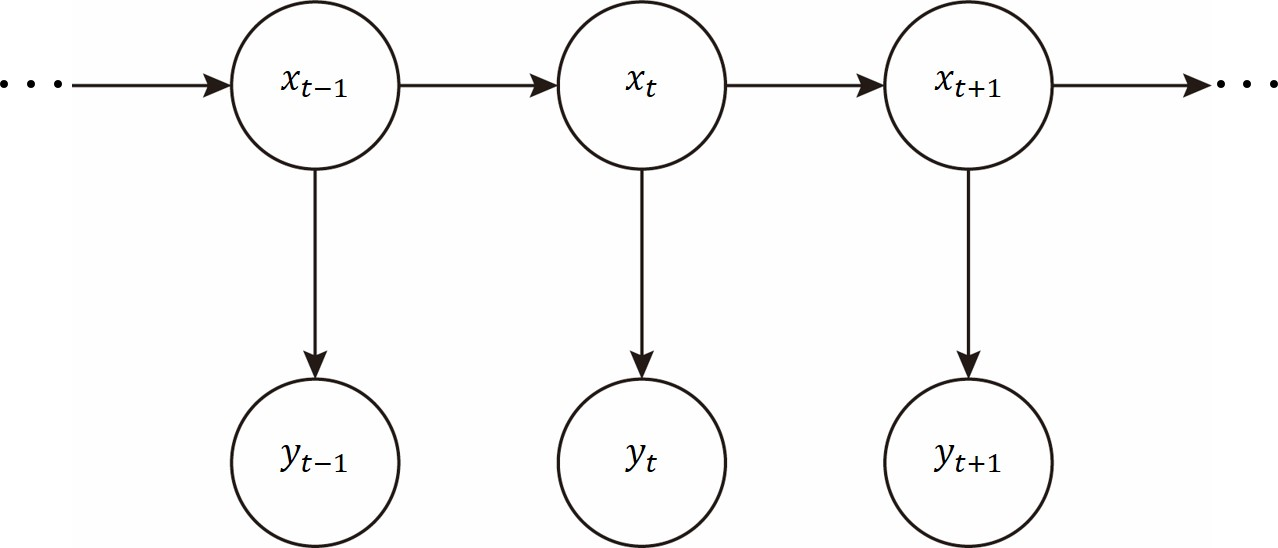
\includegraphics[width=0.65\linewidth]{SSM.jpg}
    \caption{Graphical model of an SSM with latent process $x$ and observed process $y$.}
    \label{fig:SSM}
\end{figure}

\noindent As shown in figure \ref{fig:SSM}, a state space model consists of two stochastic processes $\left\{x_{t}\right\}_{t \geq 1}$ and $\left\{y_{t}\right\}_{t \geq 1}$, where $x_{t}$ denotes the latent state (top) and $y_{t}$ denotes the observation (bottom) from the system at time t. We assume that the states and observations are real-valued, i.e., $y_{t} \in \mathcal{Y} \subseteq \mathbb{R}^{n_{y}}$ and $x_{t} \in \mathcal{X} \subseteq\mathbb{R}^{n_{x}}$. The latent state $\left\{x_{t}\right\}_{t \geq 1}$ is modelled as a first-order Markov process of initial density $\mu_{\theta}(x)$, i.e., the latent state $x_{t}$ only depends on the previous state $x_{t-1}$. That is, all the information in the past states $x_{1: t-1} \triangleq\left\{x_{s}\right\}_{s=1}^{t-1}$ is summarized in the most recent state $x_{t-1}$. The observations $y_{1:t}$ are conditionally independent as the observation $y_{t}$ is only related to the corresponding state  $x_{t}$.\\

\noindent The densities of the latent state and the observation process are 
$f_{\theta}\left(x_{t} \mid x_{t-1}\right)$ and $g_{\theta}\left(y_{t} \mid x_{t}\right)$, respectively, where $\theta \in \Theta \subset \mathbb{R}^{p}$ is the unknown parameter vector.
The density $f_{\theta}\left(x_{t} \mid x_{t-1}\right)$ describes the probability that the next state is $x_{t}$ given the previous state $x_{t-1}$. And for the observation process, $g_{\theta}\left(y_{t} \mid x_{t}\right)$ describes the 
probability that the observation is $y_{t}$ given the state $x_{t}$. Therefore, with the notation in place, a
general SSM can be expressed as
\begin{equation}\label{density}
x_{1} \sim \mu_{\theta}\left(x_{1}\right), \quad x_{t}\left|x_{t-1} \sim f_{\theta}\left(x_{t} \mid x_{t-1}\right), \quad y_{t}\right| x_{t} \sim g_{\theta}\left(y_{t} \mid x_{t}\right)\end{equation}\\


\noindent Here are some examples of state space models.
\begin{enumerate}
    \item ARMA Model\\
    The general $ARMA(p,q)$ model is
    \begin{equation}y_{t}=\phi y_{t-1}+\cdots \phi_{p} y_{t-p}+\eta_{t}+\theta_{1} \eta_{t-1}+\cdots+\theta_{q} \eta_{t-q}\end{equation}
    where $\eta_{t}$ is white noise. Let $m = max(p, q + 1)$, then
    we can rewrite the $ARMA(p,q)$ model as
    \begin{equation}y_{t}=\phi y_{t-1}+\cdots \phi_{p} y_{t-m}+\eta_{t}+\theta_{1} \eta_{t-1}+\cdots+\theta_{m-1} \eta_{t-m+1}\end{equation}
    where some of the AR or MA coefficients will be zero unless $p = q + 1$. Define $x_{t}$ as
    \begin{equation}x_{t}=\left[\begin{array}{c}
    y_{t} \\
    \phi_{2} y_{t-1}+\cdots+\phi_{p} y_{t-m+1}+\theta_{1} \eta_{t}+\cdots+\theta_{m-1} \eta_{t-m+2} \\
    \vdots \\
    \phi_{m} y_{t-1}+\theta_{m} \eta_{t}
    \end{array}\right]\end{equation}
    Then the $ARMA(p,q)$ model can be put in state space form:
    \begin{equation}x_{t}=\left[\begin{array}{ccccc}
    \phi_{1} & 1 & 0 & \cdots & 0 \\
    \phi_{2} & 0 & 1 & \cdots & 0 \\
    \vdots & \vdots & \vdots & \ddots & \vdots \\
    \phi_{m-1} & 0 & 0 & \cdots & 1 \\
    \phi_{m} & 0 & 0 & \cdots & 0
    \end{array}\right] x_{t-1}+\left[\begin{array}{c}
    1 \\
    \theta_{1} \\
    \vdots \\
    \theta_{m-2} \\
    \theta_{m-1}
    \end{array}\right] \eta_{t}\\
    \end{equation}
    \begin{equation}
    y_{t}=\left[\begin{array}{ccccc}1 & 0 & 0 & \cdots & 0\end{array}\right] x_{t} 
    \end{equation}
 
    
    
    \item Time Varying Parameter Model\\
    A time varying parameter model can be used to simulate financial markets. The general model is:
    \begin{equation}\begin{array}{c}
    R_{t}=\alpha_{t}+\beta_{t} R_{m t}+v_{t} \\
    \alpha_{t}=\alpha_{t-1}+w_{1 t}, \quad w_{1 t} \sim N\left(0, \sigma_{1}^{2}\right) \\
    \beta_{t}=\beta_{t-1}+w_{2 t},  \quad w_{2 t} \sim N\left(0, \sigma_{2}^{2}\right)
    \end{array}\end{equation}
    where $R_{t}$ is our return on assets and $R_{mt}$ is the market interest rate. 
    Define $x_{t}$ as :
    \begin{equation}x_{t}=\left[\begin{array}{l}
    \alpha_{t} \\
    \beta_{t}
    \end{array}\right]\end{equation}
    Then the time varying parameter model can be written as a state space model:
    \begin{equation}\begin{array}{c}
    x_{t}=\left[\begin{array}{cc}
    1 & 0\\
    0 & 1
    \end{array}\right] x_{t-1}+\left[\begin{array}{c}
    w_{1 t} \\
    w_{2 t}
    \end{array}\right] \\
    \end{array}
    \end{equation}
    \begin{equation}
    R_{t}=\left[1\quad R_{m t}\right] x_{t}+v_{t}
    \end{equation}
    
\end{enumerate}
An overview of some concrete applications in many other fields including earthquake counts, polio counts, rainfall occurrence data, glacial varve data and daily returns on a share can be seen in \cite{langrock2011some}.

\section{Inference Problems for State Space Model}
\noindent  There are often two different inference problems connected to SSMs: 
the state inference problem and the parameter inference problem.
The first problem is to infer the density of the latent state process given the observations and the model where the
parameter $\theta$ is known. That is, we would like to determine the value of $x_{t}$ given the information in the observations $y_{1:t}$, i.e., $p_{\theta}\left(x_{t} \mid y_{1: t}\right)$. 
The second problem is to infer the value of the parameter vector $\theta$ from the observations $y_{1: T}$. \\

\noindent Actually, parameter inference is often the primary problem of interest.
The existing inference methods
can be classified into two categories: Bayesian or Maximum Likelihood (ML). \\

\begin{enumerate}
    \item Maximum likelihood parameter inference\\
    
    The likelihood function of an
    SSM can be expressed as 
    \begin{equation}\mathcal{L}(\theta)=p_{\theta}\left(y_{1: T}\right)=p_{\theta}\left(y_{1}\right) \prod_{t=2}^{T} p_{\theta}\left(y_{t} \mid y_{1: t-1}\right).\end{equation}
    To simplify  calculations and improve the numerical stability of many algorithms, we often replace the likelihood function with the log-likelihood function given by
    \begin{equation}\ell(\theta)=\log p_{\theta}\left(y_{1: T}\right)=\log p_{\theta}\left(y_{1}\right)+\sum_{t=2}^{T} \log p_{\theta}\left(y_{t} \mid y_{1: t-1}\right).\end{equation}
    
    We regard the likelihood as a function of the parameter and thus, the parameter which maximizes the likelihood or equivalently the log-likelihood  is what we want. We should select the parameter that together
    with the model is the most likely to have been generated the observations.
    Therefore, the parameter inference problem in the ML setting is given by
    \begin{equation}\label{ML}
    \widehat{\theta}_{\mathrm{ML}}=\underset{\theta \in \Theta}{\operatorname{argmax}} \mathcal{L}(\theta)=\underset{\theta \in \Theta}{\operatorname{argmax}} \ell(\theta),\end{equation}
    Where $\widehat{\theta}_{\mathrm{ML}}$ denotes the ML parameter estimate.\\
    
    The score function and observed information matrix  also play an important role in parameter inference problems. The score function is defined as the gradient of
    the log-likelihood,
    \begin{equation}\mathcal{S}\left(\theta^{\prime}\right)=\left.\nabla \ell(\theta)\right|_{\theta=\theta^{\prime}}.\end{equation}
    The observed information matrix
    is defined as the negative Hessian of the log-likelihood,
    \begin{equation}\mathcal{J}\left(\theta^{\prime}\right)=-\left.\nabla^{2} \ell(\theta)\right|_{\theta=\theta^{\prime}}.
    \end{equation}
    \\
    
    The score function can be interpreted as the slope of the log-likelihood and the observed information matrix  
    measures the amount of information in the 
    data regarding the parameter $\theta$. Since  $\widehat{\theta}_{\mathrm{ML}}$ denotes the ML parameter estimate, the score function is zero when evaluated around this estimate and the  observed information matrix  should be positive definite.\\
    
    \item Bayesian parameter inference\\
    
    \noindent Another common method is to use Bayesian.
    Detailed introduction of Bayesian analysis can be seen in 
    \cite{berger2013statistical,robert2007bayesian}.
    Different from the  ML parameter estimate, where we assume that the true parameter
    is a specific value, here we regard the true parameter 
    as  a random variable following a specific distribution. 
    Our objective in Bayesian parameter inference is to
    infer an
    updated probability distribution called the posterior distribution given the information in the data 
    described by the likelihood $p_{\theta}\left(y_{1: T}\right)$ and prior  distribution of $\theta$ denoted $p\left(\theta\right)$.
    \begin{equation}p\left(\theta \mid y_{1: T}\right)=\frac{p_{\theta}\left(y_{1: T}\right) p(\theta)}{\int p_{\theta}\left(y_{1: T}\right) p(\theta) d \theta} \propto p_{\theta}\left(y_{1: T}\right) p(\theta).\end{equation}
\end{enumerate}

\noindent From the above, we can see that both of the two methods are dependent on the likelihood function which satisfies,
\begin{equation}p_{\theta}\left(y_{1: T}\right)=\int p_{\theta}\left(x_{1: T}, y_{1: T}\right) d x_{1: T},\end{equation}
where $p_{\theta}\left(x_{1: T}, y_{1: T}\right)$ denotes the joint density and is given from equation (\ref{density}) by,
\begin{equation}p_{\theta}\left(x_{1: T}, y_{1: T}\right)=\mu_{\theta}\left(x_{1}\right) \prod_{t=2}^{T} f_{\theta}\left(x_{t} \mid x_{t-1}\right) \prod_{t=1}^{T} g_{\theta}\left(y_{t} \mid x_{t}\right).\end{equation}

\noindent For the state inference, the  posterior density of the latent
states can also be given by Bayesian method:
\begin{equation}p_{\theta}\left(x_{1: t} \mid y_{1: t}\right)=\frac{p_{\theta}\left(x_{1: t}, y_{1: t}\right)}{p_{\theta}\left(y_{1: t}\right)}.\end{equation}
This posterior density is  useful for computing the
score vector of the log-likelihood according to 
Fisher’s identity,
\begin{equation}\begin{aligned}
\nabla_{\theta} \ell_{t}(\theta)=\int & \nabla_{\theta} \log p_{\theta}\left(x_{1: t}, y_{1: t}\right) 
& \cdot \quad p_{\theta}\left(x_{1: t} \mid y_{1:t}\right) d x_{1: t}.
\end{aligned}\end{equation}

\noindent Therefore, in theory, it seems that it is possible to do the inference from the above equations. 
For the linear Gaussian model, it is easy to check that $p_{\theta}\left(x_{1: t}, y_{1: t}\right) $ is a Gaussian distribution and Kalman filtering algorithm \cite{anderson2012optimal} is always the optimal solution of the estimation.
However, in practice, most of the problems we need to deal with are  nonlinear non-Gaussian state space models
whose likelihood function is analytically intractable and
the posterior might not be
any known distribution. As a consequence, we cannot compute many of the
integrals depending on the posterior distribution in closed-form.
To solve these problems, a number of different numerical approaches and sampling methods have been developed.
Thus, the main topic in this thesis is to deal with these problems by particle filter method, also known
as Sequential Monte Carlo (SMC) method.\\

\section{Filtering Algorithms}
\noindent According to different time series of measurements and estimates,
the inference problems in an SSM can be classified into mainly two types: filtering and smoothing.
Both the filtering and smoothing problem can be marginal (inference
on a single state), k-interval (inference of k states) or joint (inference on all states).
In filtering, only observations $y_{1:t}$  collected until the current time step
t  are used to infer the current state $x_{t}$.
Inferring the value of the current state $x_{t}$ with $t \leq T$ by using all the collected observations including (possibly) future observations $y_{1:T}$ is called smoothing.
In Table \ref{table:fs}, we can see some common filtering and smoothing problems in SSMs.



\begin{table}[H]
\centering
\begin{tabular}{ll}
\hline Name & Density \\
\hline (Marginal) filtering & $p_{\theta}\left(x_{t} \mid y_{1: t}\right)$ \\
(Marginal) smoothing $(t \leq T)$ & $p_{\theta}\left(x_{t} \mid y_{1: T}\right)$ \\
Joint smoothing & $p_{\theta}\left(x_{1: T} \mid y_{1: T}\right)$ \\
Fixed-interval smoothing $(s<t \leq T)$ & $p_{\theta}\left(x_{s: t} \mid y_{1: T}\right)$ \\
Fixed-lag smoothing (for lag $\Delta)$ & $p_{\theta}\left(x_{t-\Delta-1: t} \mid y_{1: t}\right)$ \\
\hline
\end{tabular}
\caption{Common filtering and smoothing densities in SSMs}
\label{table:fs}
\end{table}

\noindent Many different filtering algorithms have been developed to deal with these filtering and smoothing problems in SSMs.\\

\subsection{Linear Filtering Algorithms}
\noindent When we refer to optimal estimation in filtering and smoothing problems, we always means estimating the value of unknown states or parameters by some optimal chosen criterion.  
A well known method of parameter estimate was Least Squares Estimation raised by Gauss in 1795 \cite{stigler1981gauss,agrawal2018rewriting}.
Norbert Wiener proposed Wiener Filtering Algorithm in 1940s in order to solve the problem of automatic aiming and firing control of anti-aircraft artillery system problem\cite{wiener1949extrapolation}. The discrete time model of this  filtering algorithm was proposed by Andrey Nikolaevich
Kolmogorov in 1941\cite{kolmogoroff1941interpolation}.
Thus, this is often referred to as Wiener-Kolmogorov filtering
theory.  Although Wiener Filtering Algorithm is an optimal filtering algorithm for linear systems,
all the information in the past time is need in the algorithm, so it is difficult to perform on-line recursive calculation.
In 1960, this problem was solved by Kalman Filter\cite{kalman1960new}.
The KF algorithm only depends on one previous observation in the estimation procedure, easy to carry out on-line recursive calculation. And meantime, for linear Gaussian systems, KF algorithm is also an optimal filtering algorithm.
An important breakthrough here is that
State Space Model is used to define the KF algorithm, which
directly result in the wide use of State Space model later in various fields. Most nonlinear filtering algorithms are also developed from this algorithm.\\
\subsection{Nonlinear Filtering Algorithms}
\noindent However, most systems are nonlinear
in reality so that the KF  algorithm cannot be used under this situation. 
The extended Kalman filtering algorithm(EKF)\cite{bucy1971digital,sunahara1970approximate} was developed based on 
the structure of Kalman filtering algorithm.
It linearizes the nonlinear system by Taylor series expansion,
which lead to a suboptimal solution of the state variable estimation.
The extended Kalman filtering algorithm is widely used in
weak nonlinear state space models because of the high efficiency of the calculation.
But for the system with high nonlinearity, the linearization process makes the result not accuracy enough as the higher order terms of Taylor series expansion cannot be ignored directly.
What's more, higher order
Taylor series expansion needs more computing resources and will
make the algorithm inefficient.\\

\noindent Another approximation method is called Unscented Kalman Filter(UKF) which is developed based on Unscented Transform(UT) \cite{julier1997new}. This algorithm improves the calculation accuracy to some extent 
in comparison to EKF. 
However, the EKF and UKF algorithms  both are only applicable to the systems where the noises  follow the Gaussian distribution.
Other nonlinear filtering algorithms include Central Difference Kalman Filter(CDKF), Divided Difference Kalman Filter(DDKF) and
Quadrature Kalman Filter(QKF).\\

\subsection{Monte Carlo Approximation}
\noindent In order to work on non-Gaussian noise, a Particle Filter (PF) algorithm based on Sequential Monte Carlo (SMC) structure called Bootstrap Filter was created in 1993 \cite{gordon1993novel}. This is the important milestone for the later rapid development of particle filter.
The PF algorithm uses a set of weighted samples (also called particles)  to represent the posterior distribution of the random process given noise and observations. 
The  estimation of unknown variables is realized by recursively calculating and adjusting the weights of the particles. \\

\noindent The predecessor of the PF algorithm is the Monte Carlo (MC) method based on Sequential Importance Sampling (SIS). 
The MC integration method based on SIS was used in physics and statistics in 1950s \cite{hammersley1954poor}.
However, this method had not been fully and effectively developed for a long period of time because of the particle degeneracy problem in SIS until Bootstrap Filter appeared.
The solution is to add resampling process to the algorithm and thus the SIS method is improved to Sequential Importance Resampling method(SIR).
However, SIR also leads to  Sample Impoverishment problem, which means too-few samples at a certain moment.
There are many methods to improve the PF algorithm around these issues , including 
choosing better importance density function, getting suitable resampling method, etc.






\chapter{State Inference Using Particle Methods}

%%%%%%%%%%%%%%%%%%%%%%%%%%%%%%%%%%%%%

\noindent In this chapter we assume the parameter $\theta$ is known
and we focus on the problem of estimating the latent
process $\left\{x_{t}\right\}_{t \geq 1}$ 
sequentially given the observations.
The estimation process also 
provides us with an on-line scheme to compute
 $\left\{p_{\theta}\left(y_{1:t}\right)\right\}_{t \geq 1}$.
The particle
approximation of these  terms are the main topic to be discussed
in this chapter.



\section{Recursive Bayesian Estimation}
\noindent Generally speaking, regardless of linear systems or nonlinear systems, the optimal filtering problem can be solved
by recursive Bayesian estimation \cite{ho1964bayesian}.
The key idea of recursive Bayesian estimation  is to 
estimate the posterior probability density function
based on prior knowledge and data information.
The complete algorithm often consists of two steps:
the prediction process and the update process.\\

\noindent To simplify the problem, we first consider
the task of estimating recursively
in time the sequence of marginal posteriors 
$\left\{p\left(x_{t} \mid y_{1: t}\right)\right\}_{t \geq 1}$.
Assume that the posterior probability density
$p\left(x_{t-1} \mid y_{1:t-1}\right)$ is known, then
the process of recursive Bayesian estimation is as follows:\\
\begin{enumerate}
    \item Prediction: we predict $p\left(x_{t} \mid y_{1:t-1}\right)$ from $p\left(x_{t-1} \mid y_{1:t-1}\right)$. 
    According to Chapman-Kolmogorov Equation, we can have
    \begin{equation}\label{Prediction}
        p\left(x_{t} \mid y_{1:t-1}\right)=\int p\left(x_{t} \mid x_{t-1}\right) p\left(x_{t-1} \mid y_{1:t-1}\right) d x_{t-1},
    \end{equation}
    where $p\left(x_{t} \mid x_{t-1}\right)$ is
    the Markov state transition density function $f_{\theta}\left(x_{t} \mid x_{t-1}\right)$ which is decided
    by the model.\\
    
    \item Update: we update 
    $p\left(x_{t} \mid y_{1:t}\right)$ when we have new observation at time $t$. By Bayes' theorem, we have\\
    \begin{equation}\begin{aligned}
    p\left(x_{t}\mid y_{1:t} \right) &=\frac{p\left(y_{1:t} \mid x_{t}\right) p\left(x_{t}\right)}{p\left(y_{1:t}\right)} \\
    &=\frac{p\left(y_{t}, y_{1:t-1}\mid x_{t}\right) p\left(x_{t}\right)}{p\left(y_{t}, y_{1:t-1}\right)}
    \\
    &=\frac{p\left(y_{t} \mid y_{1:t-1}, x_{t}\right) p\left(y_{1: t-1}\mid x_{t}\right) p\left(x_{t}\right)}{p\left(y_{t} \mid y_{1: t-1}\right) p\left(y_{1: t-1}\right)}
    \\
    &=\frac{p\left(y_{t} \mid y_{1: t-1}, x_{t}\right) p\left(x_{t} \mid y_{1: t-1}\right) p\left(y_{1: t-1}\right) p\left(x_{t}\right)}{p\left(y_{t} \mid y_{1: t-1}\right) p\left(y_{1: t-1}\right) p\left(x_{t}\right)}
    \\
    &=\frac{p\left(y_{t} \mid y_{1:t-1}, x_{t}\right) p\left(x_{t} \mid y_{1: t-1}\right)}{p\left(y_{t} \mid y_{1: t-1}\right)}
    \end{aligned}\end{equation}
    \noindent Since the observations $y_{1:t}$ are conditionally independent, we can have
    \begin{equation}
        p\left(y_{t} \mid y_{1:t-1}, x_{t}\right)=
        p\left(y_{t} \mid x_{t}\right).
    \end{equation}
    \noindent Therefore, the posterior distribution can be
    written as 
    \begin{equation}\label{update}
    \begin{aligned}
        p\left(x_{t}\mid y_{1:t} \right) &=
        \frac{p\left(y_{t} \mid  x_{t}\right) p\left(x_{t} \mid y_{1: t-1}\right)}{p\left(y_{t} \mid y_{1: t-1}\right)},
    \end{aligned}
    \end{equation}
    where $p\left(y_{t} \mid  x_{t}\right)$ is defined in
    the model by $g_{\theta}\left(y_{t} \mid x_{t}\right)$,
    and $p\left(y_{t} \mid y_{1: t-1}\right)$ is the
    normalizing constant
    \begin{equation}
        p\left(y_{t} \mid y_{1: t-1}\right)=
        \int p\left(y_{t} \mid x_{t}\right) p\left(x_{t} \mid y_{1: t-1}\right) \mathrm{d} x_{t}.
    \end{equation}
\end{enumerate}

\begin{figure}[H]
    \centering
    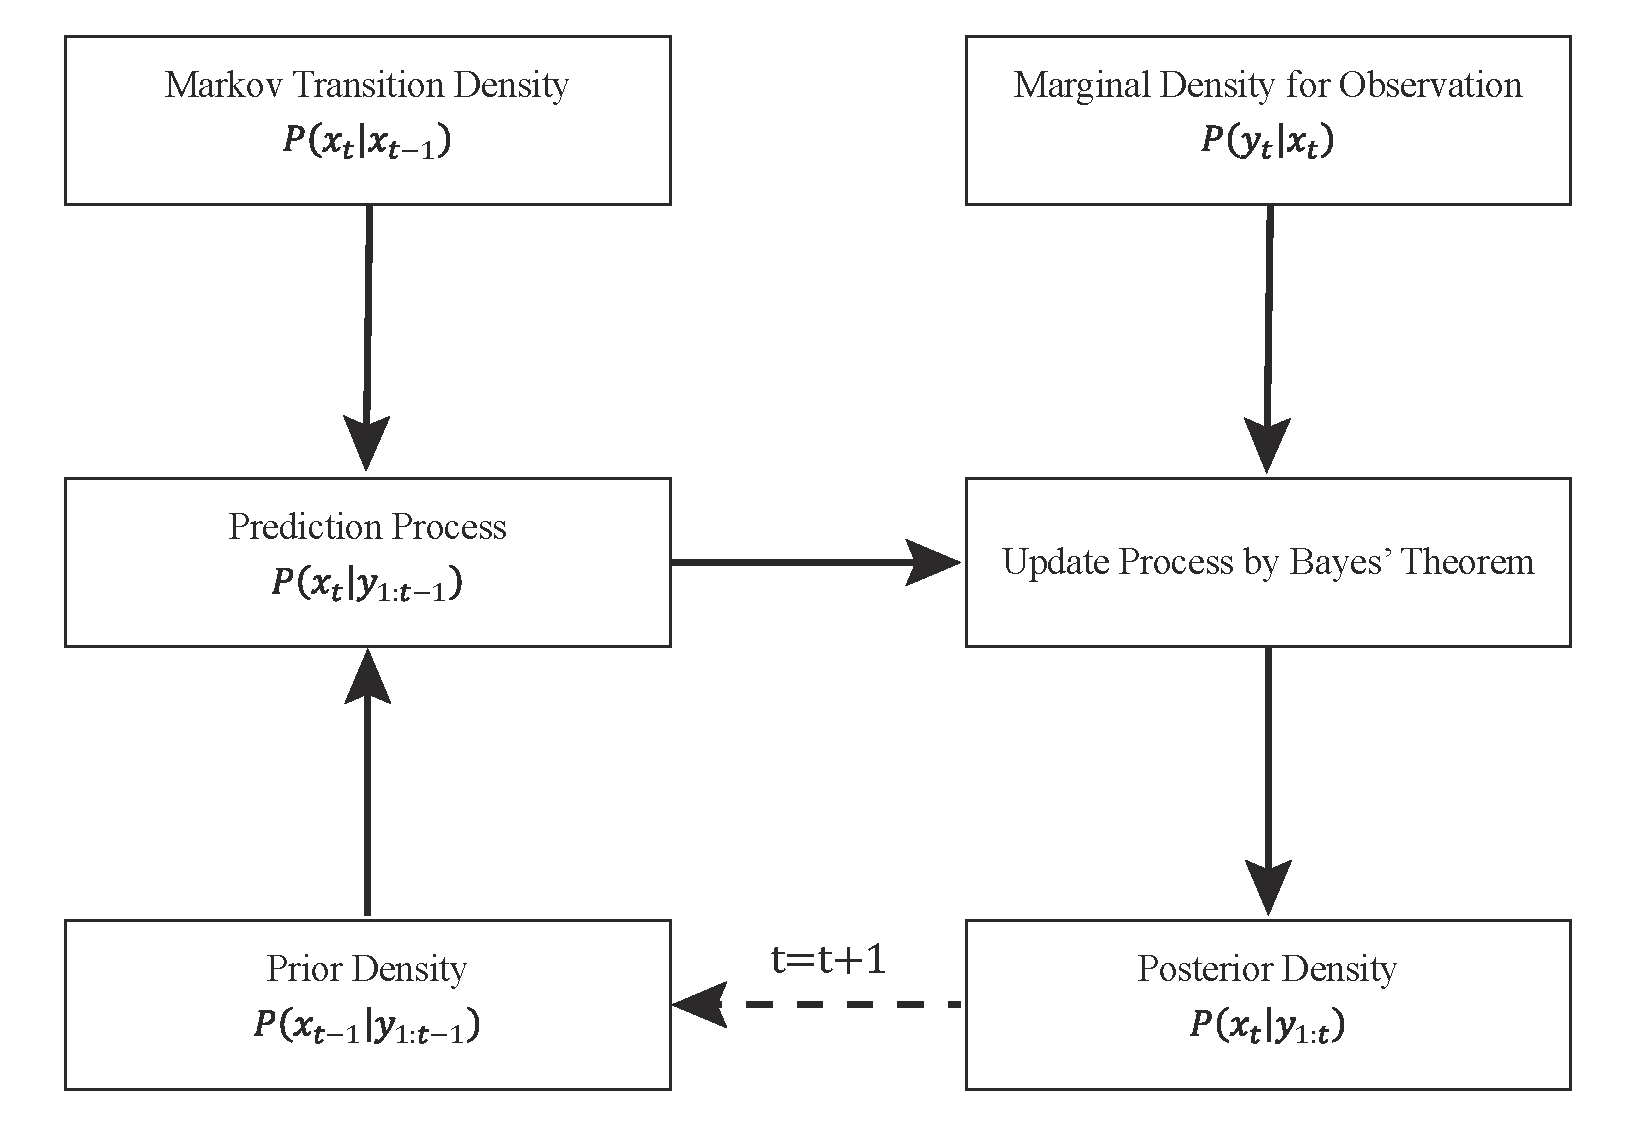
\includegraphics[width=0.80\linewidth]{pau.pdf}
    \caption{ Process of the recursive Bayesian estimation.}
    \label{fig:pau}
\end{figure}

\noindent Therefore, we have completed the recursive Bayesian estimation process as shown in Figure \ref{fig:pau}\\



\noindent In a similar manner, the smoothing problem can be solved by
\begin{equation}p\left(x_{t+1} \mid y_{1: t}\right)=\int p\left(x_{t+1} \mid x_{t}\right) p\left(x_{t} \mid y_{1: t}\right) \mathrm{d} x_{t},\end{equation}
\begin{equation}p\left(x_{t} \mid y_{1: T}\right)=p\left(x_{t} \mid y_{1: t}\right) \int \frac{p\left(x_{t+1} \mid x_{t}\right) p\left(x_{t+1} \mid y_{1: T}\right)}{p\left(x_{t+1} \mid y_{1: t}\right)} \mathrm{d} x_{t+1}.\end{equation}\\

\noindent Since $p\left(x_{t}\mid y_{1:t} \right)$
is the marginal density of posterior density 
$p\left(x_{1:t}\mid y_{1:t} \right)$, the general equation
of joint posterior density obtained by recursive Bayesian estimation
is 
\begin{equation}\label{re}
p\left(x_{1:t} \mid y_{1:t}\right)
=p\left(x_{1:t-1} \mid y_{1:t-1}\right) \frac{p\left(x_{t} \mid x_{t-1}\right) p\left(y_{t} \mid x_{t}\right)}{p\left(y_{t} \mid y_{1:t-1}\right)},
\end{equation}
where the normalizing constant is 
\begin{equation}\label{y}
    p\left(y_{t} \mid y_{1: t-1}\right)=
    \int p\left(x_{1:t-1} \mid y_{1:t-1}\right)
    p\left(x_{t} \mid x_{t-1}\right) p\left(y_{t} \mid x_{t}\right) \mathrm{d} x_{1:t}.
\end{equation}

\noindent Equation (\ref{Prediction}) is known as the prediction step and (\ref{update}) is known as the update step. However, most
particle filtering methods rely on a numerical approximation of recursion (\ref{re}) and not of (\ref{Prediction}) and (\ref{update}).\\

\noindent If we can compute ${p\left(x_{1:t} \mid y_{1:t}\right)}$
and thus ${p\left(x_{t} \mid y_{1:t}\right)}$ sequentially, then the  marginal likelihood $p\left(y_{1:t}\right)$
can also clearly be evaluated recursively using
\begin{equation}\label{likelihood}
p\left(y_{1: t}\right)=p\left(y_{1}\right) \prod_{k=2}^{t} p\left(y_{k} \mid y_{1: k-1}\right)
\end{equation}
where $p\left(y_{k} \mid y_{1: k-1}\right)$ is of the form (\ref{y}).\\



\noindent Actually, the recursive process
is the general framework of the filtering algorithms.
Yu-Chi Ho and Robert C. K. Lee first studied on the 
recursive Bayesian filtering problem and
pointed that Kalman filtering algorithm is 
a special case of Bayesian filtering\cite{ho1964bayesian}.
As we discussed before, the recursions can only be solved analytically
for two different classes of SSMs: 
linear Gaussian SSMs and SSMs with finite state
processes.  
For the former, the recursions can be
implemented using Kalman filter (KF).\\

\noindent If the system does not satisfy the linear Gaussian condition,
it is difficult to obtain the analytical solution of Bayesian filtering. Two main methods are used to solve  nonlinear systems.
One is the analytical approximation for models with Gaussian noise, such as the EKF discussed in
chapter \ref{s-intro}.
The other method 
is simulation approximation based on Monte Carlo when noise is non-Gaussian, such as the Particle Filter(PF) method we will discuss later. 
Figure \ref{fig:bf} shows the classification of Bayesian filtering.\\

\begin{figure}[H]
    \centering
    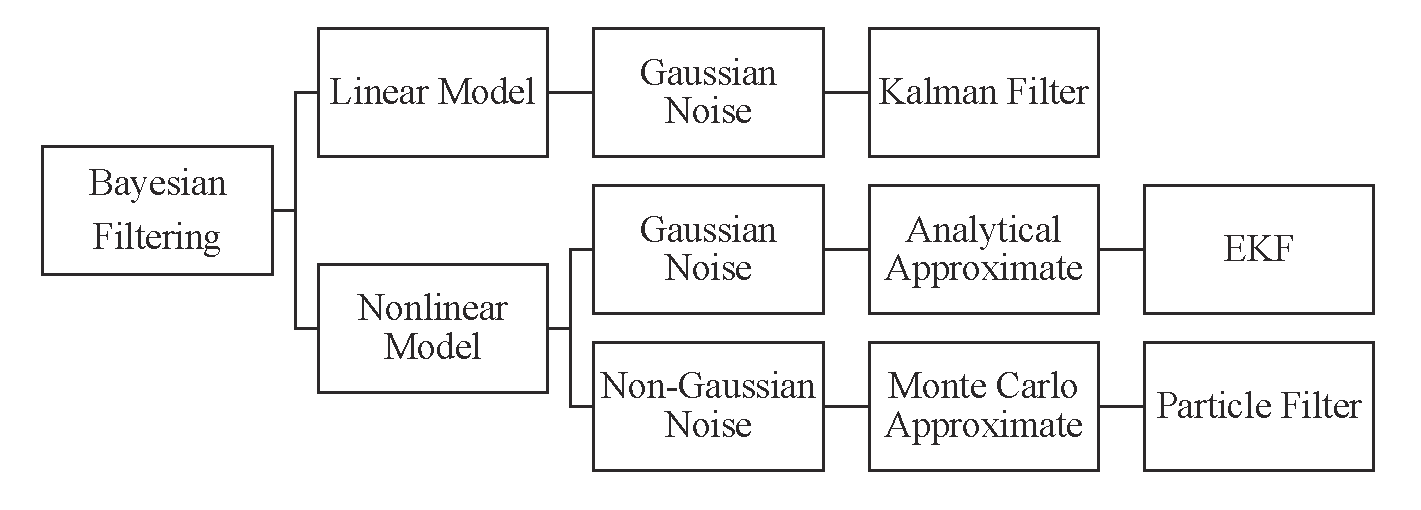
\includegraphics[width=0.90\linewidth]{bf.pdf}
    \caption{Classification of Bayesian filtering.}
    \label{fig:bf}
\end{figure}








\section{Monte Carlo and Importance Sampling}
\noindent Generally speaking, the Particle Filter method 
can be seen as the application of Monte Carlo method in Bayesian estimation and
is accessible to any nonlinear system which can be described by State Space model.  
Since PF algorithm is developed from the Monte Carlo (MC) method based on Sequential Importance Sampling (SIS) and improved by Sequential Importance Resampling method(SIR), we will introduce PF starting from
MC method and importance sampling in this section.\\

\subsection{Monte Carlo method}
\noindent MC methods are a collection of statistical simulation methods based on sampling
and the strong law of large numbers (SLLN).
The idea is to use a large number of sample points in the state space to approximate the posterior probability distribution function of the variable.
As shown in Figure \ref{fig:mc}, the circles in the figure represent discrete sample points, thus the integration problem is transformed into a summation problem of finite sample points.\\


\begin{figure}
    \centering
    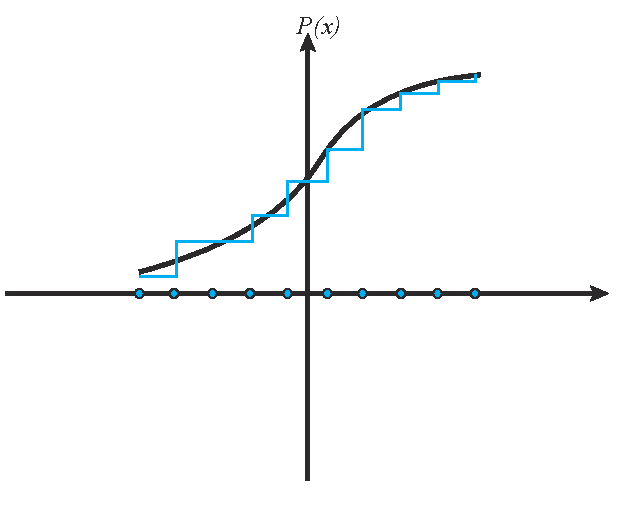
\includegraphics[width=0.50\linewidth]{mc.pdf}
    \caption{MC method for integration problem.}
    \label{fig:mc}
\end{figure}

\noindent Here, we consider estimating
the expected value (an integral) of a function $\varphi(x)$
\begin{equation}\widehat{\varphi}=\mathbb{E}_{\pi}[\varphi(x)]=\int \varphi(x) \pi(x) \mathrm{d} x\end{equation}
where $\pi(x)$  denotes a (normalised)  distribution that
$x$ follows.
If we can sample a set of independently identically distribution(IID) particles $\left\{x_{1}, x_{2}, \cdots, x_{N}\right\}$ from $\pi(x)$, as a consequence of the SLLN,
we can estimate the
expectation by the sample average
\begin{equation}\widehat{\varphi}_{\mathrm{MC}}=\frac{1}{N} \sum_{i=1}^{N} \varphi\left(x^{(i)}\right), \quad x^{(i)} \sim \pi(x).\end{equation}\\

\noindent Similarly, for Bayesian filtering problem, we can sample 
IID particles $\left\{x_{1:t}^{i}\right\}_{i=1}^{N}$
from  posterior probability density $p\left(x_{1:t} \mid y_{1:t}\right)$.
Then the posterior probability density can be approximated by the following formula,
\begin{equation}\hat{p}\left(x_{1:t} \mid y_{1:t}\right)=\frac{1}{N} \sum_{i=1}^{N} \delta\left(x_{1:t}-x_{1:t}^{\left(i\right)}\right),\end{equation}
where $\delta(\cdot)$ is Dirac-delta function defined by
\begin{equation}\delta(x)=\left\{\begin{array}{ll}
+\infty, & x=0 \\
0, & x \neq 0
\end{array}\right.\end{equation}
and is also constrained to satisfy the identity,
\begin{equation}\int_{-\infty}^{\infty} \delta(x) d x=1.\end{equation}
Based on this approximation, the conditional expectation of function $\varphi(x_{1:t})$ 
\begin{equation}E\left[\varphi\left(x_{1:t}\right)\right]=\int \varphi\left(x_{1:t}\right) p\left(x_{1:t} \mid y_{1:t}\right) d x_{1:t}\end{equation}
can be approximated by
\begin{equation}\begin{aligned}
\hat{E}\left[\varphi\left(x_{1:t}\right)\right] &=\frac{1}{N} \sum_{i=1}^{N} \int \varphi\left(x_{1:t}\right) \delta\left(x_{1:t}-x_{1:t}^{\left(i\right)}\right) d x_{1:t} \\
&=\frac{1}{N} \sum_{i=1}^{N} \varphi\left(x_{1:t}^{\left(i\right)}\right)
\end{aligned}\end{equation}

\noindent The convergence of this estimator is guaranteed by
SLLN, i.e.
\begin{equation}
\hat{E}\left[\varphi\left(x_{1:t}\right)\right] \stackrel{a . s}{\longrightarrow} \E\left[\varphi\left(x_{1:t}\right)\right], \quad N \rightarrow \infty.\end{equation}\\

\noindent Therefore, in theory, we can use the mean value of the sample particles to estimate the expectation.
The main advantage of Monte Carlo methods  is that the variance of
the approximation error decreases at a rate of
$\mathcal{O}(1 / N)$ regardless of the dimension of the space. However, the problem of this approach is also obvious.
Since we don’t know the posterior probability density
$p\left(x_{1:t} \mid y_{1:t}\right)$, we certainly cannot
directly sample from it.
In this case, importance
sampling (IS) \cite{marshall1954use} can be used to sample from another distribution
called the proposal distribution (or importance distribution) $q\left(x_{1:t} \mid y_{1:t}\right)$ and adapt the
particles using a weighting scheme.\\

\subsection{Importance Sampling}
\noindent Importance sampling is 
the basis of all the algorithms developed later on.
By using the particle system $\left\{w_{t}^{(i)}, x_{t}^{(i)}\right\}_{i=1}^{N}$, where $x_{t}^{(i)}$ and
$w_{t}^{(i)}$ denote particle
i at time t and its corresponding (unnormalised) importance weight, we can approximate the posterior probability density by
\begin{equation}\widehat{p}\left( x_{1:t} \mid y_{1: t}\right) \triangleq \sum_{i=1}^{N} \widetilde{w}_{t}^{(i)} \delta\left( x_{1:t}-x_{1:t}^{(i)}\right)\end{equation}\\
\begin{equation}\widetilde{w}_{t}^{(i)} \triangleq \frac{w_{t}^{(i)}}{\sum_{k=1}^{N} w_{t}^{(k)}}.\end{equation}\\

\noindent In practice, sampling from posterior probability density is impossible, so we need an
importance distribution $q\left(x_{1:t} \mid y_{1:t}\right)$
which is easily to be sampled from.
To see how it works, first we rewrite  the conditional expectation of function
$\varphi(x_{1:t})$  as 
\begin{equation}\begin{aligned}
E\left[\varphi\left(x_{1:t}\right)\right]&=\int \varphi\left(x_{1:t}\right) p\left(x_{1:t} \mid y_{1:t}\right) d x_{1:t}\\
&=\int \varphi\left(x_{1:t}\right)\frac{ p\left(x_{1:t} \mid y_{1:t}\right)}{q\left(x_{1:t} \mid y_{1:t}\right)} q\left(x_{1:t} \mid y_{1:t}\right) d x_{1:t}\\
&=\int \varphi\left(x_{1:t}\right)\frac{ p\left(y_{1:t} \mid x_{1:t}\right)p\left(x_{1:t}\right)}{q\left(x_{1:t} \mid y_{1:t}\right)p\left(y_{1:t}\right)} q\left(x_{1:t} \mid y_{1:t}\right) d x_{1:t}\\
&=\int \varphi\left(x_{1:t}\right)\frac{w_{t}\left(x_{1:t}\right) }{p\left(y_{1:t} \right)} q\left(x_{1:t} \mid y_{1:t}\right) d x_{1:t}
\end{aligned}\end{equation}
where $w_{t}\left(x_{1:t}\right)$ denotes the weight of particle $x_{1:t}$ and is in the form
\begin{equation}\begin{aligned}
w_{t}\left(x_{1:t}\right)&=
\frac{ p\left(y_{1:t} \mid x_{1:t}\right)p\left(x_{1:t}\right)}{q\left(x_{1:t} \mid y_{1:t}\right)}\\
&=\frac{ p\left(x_{1:t} \mid y_{1:t}\right)p\left(y_{1:t}\right)}{q\left(x_{1:t} \mid y_{1:t}\right)}\\
&\propto \frac{ p\left(x_{1:t} \mid y_{1:t}\right)}{q\left(x_{1:t} \mid y_{1:t}\right)}.
\end{aligned}\end{equation}\\

\noindent If we write $p\left(y_{1:t}\right)$ in the following integral,
\begin{equation}
    p\left(y_{1:t}\right)=
    \int p\left(y_{1:t} \mid x_{1:t}\right)p\left(x_{1:t}\right) d x_{1:t}
\end{equation}
then  the conditional expectation of function $\varphi(x_{1:t})$ can be transformed to the ratio of 
two expectations on distribution $q\left(x_{1:t} \mid y_{1:t}\right)$.
The detailed process of deduction is as follows.
\begin{equation}\begin{aligned}
E\left[\varphi\left(x_{1:t}\right)\right]
&=\int \varphi\left(x_{1:t}\right)\frac{w_{t}\left(x_{1:t}\right) }{p\left(y_{1:t} \right)} q\left(x_{1:t} \mid y_{1:t}\right) d x_{1:t}\\
&=\frac{1}{p\left(y_{1:t} \right)}\int \varphi\left(x_{1:t}\right)w_{t}\left(x_{1:t}\right) q\left(x_{1:t} \mid y_{1:t}\right) d x_{1:t}\\
&=\frac{\int \varphi\left(x_{1:t}\right)w_{t}\left(x_{1:t}\right) q\left(x_{1:t} \mid y_{1:t}\right) d x_{1:t}}{\int p\left(y_{1:t} \mid x_{1:t}\right)p\left(x_{1:t}\right) d x_{1:t}}\\
&=\frac{\int \varphi\left(x_{1:t}\right)w_{t}\left(x_{1:t}\right) q\left(x_{1:t} \mid y_{1:t}\right) d x_{1:t}}{\int w_{t}\left(x_{1:t}\right)q\left(x_{1:t} \mid y_{1:t}\right)d x_{1:t}}\\
&=\frac{E_{q}\left[ \varphi\left(x_{1:t}\right)w_{t}\left(x_{1:t}\right)\right]}
{E_{q}\left[ w_{t}\left(x_{1:t}\right)\right]}
\end{aligned}\end{equation}\\

\noindent Therefore, now we can sample 
IID particles $\left\{x_{1:t}^{i}\right\}_{i=1}^{N}$
from importance distribution 
$q\left(x_{1:t} \mid y_{1:t}\right)$ and apply the MC method
to get
\begin{equation}\hat{q}\left(x_{1:t} \mid y_{1:t}\right)=\frac{1}{N} \sum_{i=1}^{N} \delta\left(x_{1:t}-x_{1:t}^{\left(i\right)}\right),\end{equation}
and 
\begin{equation}\begin{aligned}
 \hat{E}\left[\varphi\left(x_{1: t}\right)\right]&=\frac{\frac{1}{N} \sum_{i=1}^{N} \varphi\left(x_{1: t}^{(i)}\right) w_{t}\left(x_{1: t}^{(i)}\right)}{\frac{1}{N} \sum_{i=1}^{N} w_{t}\left(x_{1: t}^{(i)}\right)}  \\
 &=\sum_{i=1}^{N} \varphi\left(x_{1: t}^{(i)}\right)
 \frac{w_{t}\left(x_{1: t}^{(i)}\right)}{ \sum_{i=1}^{N} w_{t}\left(x_{1: t}^{(i)}\right)}\\
 &=\sum_{i=1}^{N} \varphi\left(x_{1:t}^{(i)}\right) \tilde{w}_{t}\left(x_{1:t}^{(i)}\right),
\end{aligned}\end{equation}
where $\tilde{w}_{t}\left(x_{1:t}^{(i)}\right)$ is the normalized importance weight, given by
\begin{equation}\label{nweight}\widetilde{w}_{t}\left(x_{1:t}^{(i)}\right)
=\frac{w_{t}\left(x_{1: t}^{(i)}\right)}{ \sum_{i=1}^{N} w_{t}\left(x_{1: t}^{(i)}\right)}
\triangleq \widetilde{w}_{t}^{(i)} \quad i=1, \ldots, N\end{equation}
and satisfies
\begin{equation}\tilde{w}_{t}^{i} \in[0,1],
\quad \sum_{i=1}^{N} \tilde{w}_{t}^{i}=1.
\end{equation}\\

\subsection{Sequential Importance Sampling}
In the method of importance sampling, all the observation data until the current time step $t$  are required to  estimate the posterior probability density.  
That is, when new observation data arrives, the importance weight of the entire state sequence needs to be recalculated again.
Thus, to avoid the computational complexity, we can
apply the sequential analysis to MC method to achieve a
recursive algorithm called Sequential Importance Sampling(SIS).\\

\noindent This solution involves selecting an importance
distribution which has the following structure\\
\begin{equation}\begin{aligned}
q\left( x_{1:t} \mid y_{1:t}  \right)
&=q\left( x_{t} \mid x_{1:t-1},y_{1:t}  \right)q\left( x_{1:t-1} \mid y_{1:t}  \right)\\
&=q\left( x_{t} \mid x_{1:t-1},y_{1:t}  \right)q\left( x_{1:t-1} \mid y_{1:t-1}  \right).
\end{aligned}\end{equation}\\
From equation (\ref{re}) we have,
\begin{equation}
p\left(x_{1:t} \mid y_{1:t}\right)
\propto p\left(x_{1:t-1} \mid y_{1:t-1}\right) p\left(x_{t} \mid x_{t-1}\right) p\left(y_{t} \mid x_{t}\right).
\end{equation}\\
\noindent Thus, the associated unnormalised weights can be computed
recursively using the decomposition
\begin{equation}\label{weight}\begin{aligned}
w_{t}^{(i)} &\propto \frac{ p\left(x_{1:t}^{(i)} \mid y_{1:t}\right)}{q\left(x_{1:t}^{(i)} \mid y_{1:t}\right)} \\
&\propto \frac{p\left(x_{1:t-1}^{(i)} \mid y_{1:t-1}\right) p\left(x_{t}^{(i)} \mid x_{t-1}^{(i)}\right) p\left(y_{t} \mid x_{t}^{(i)}\right)}{q\left( x_{t}^{(i)} \mid x_{1:t-1}^{(i)},y_{1:t}  \right)q\left( x_{1:t-1}^{(i)} \mid y_{1:t-1}  \right)}\\
&=w_{t-1}^{(i)} \frac{ p\left(x_{t}^{(i)} \mid x_{t-1}^{(i)}\right) p\left(y_{t} \mid x_{t}^{(i)}\right)}{q\left( x_{t}^{(i)} \mid x_{1:t-1}^{(i)},y_{1:t}  \right)}.
\end{aligned}\end{equation}\\

\noindent To choose a suitable importance distribution, 
we assume $q\left( x_{t}^{(i)} \mid x_{1:t-1}^{(i)},y_{1:t}  \right)=q\left( x_{t}^{(i)} \mid x_{t-1}^{(i)},y_{t}  \right)$,
then equation (\ref{weight})
can be written as
\begin{equation}
w_{t}^{(i)} \propto
w_{t-1}^{(i)} \frac{ p\left(x_{t}^{(i)} \mid x_{t-1}^{(i)}\right) p\left(y_{t} \mid x_{t}^{(i)}\right)}{q\left( x_{t}^{(i)} \mid x_{t-1}^{(i)},y_{t}  \right)}.
\end{equation}\\
The normalised weight $\widetilde{w}_{t}^{(i)}$ is calculated by equation (\ref{nweight}).
And the posterior  probability  density can be approximated by
\begin{equation}\hat{p}\left(x_{t} \mid y_{1: t}\right) = \sum_{i=1}^{N} \tilde{w}_{t}^{(i)} \delta\left(x_{t}-x_{t}^{(i)}\right).\end{equation}\\

\noindent So far, we have completed the process of SIS algorithm.
We randomly sample particles from the proposal distribution,
sequentially calculate the corresponding importance weight
of particles according to equation (\ref{weight}), 
and finally approximate the posterior probability distribution of the system state in the form of  weighted summation of particles, so as to get the recursive estimate of state expectation:
\begin{equation}\hat{x}_{t}=\sum_{i=1}^{N} x_{t}^{(i)} \cdot \tilde{w}_{t}^{(i)}.\end{equation}\\

\noindent In the classical bootstrap particle
filter algorithm, the Markov transition density
$p\left( x_{t} \mid x_{t-1}\right)$
is chosen to be
the proposal distribution, i.e.
\begin{equation}
 q\left( x_{t}^{(i)} \mid x_{t-1}^{(i)},y_{t}\right)
 =p\left( x_{t}^{(i)} \mid x_{t-1}^{(i)}\right).
\end{equation}\\

\noindent Thus the importance weight is calculated sequentially by
\begin{equation}
w_{t}^{(i)} \propto
w_{t-1}^{(i)}   p\left(y_{t} \mid x_{t}^{(i)}\right).
\end{equation}\\

\subsection{Resampling}
\noindent It appears that we have provided a feasible solution to the filtering problem, however, it is important to be aware that the method presented here suffers from severe drawbacks.
The main problem of this algorithm is that the variance of the estimate increases exponentially with $t$ \cite{kong1994sequential}.
This results from that the particle weights deteriorate over time
and in the limit most particle weights become very small (almost zero) after a few iterations.
Hence, many ineffective number of particles consume a lot of computational resources but contribute a little to the posterior estimate, even influence the accuracy of the algorithm.
This phenomenon is called Particle Degeneracy.\\

\noindent Resampling techniques are a key ingredient of SMC methods which  solve particle degeneracy problem in
some important scenarios.
By including a resampling step into the SIS algorithm, we can  focus the computational efforts
on the “promising” regions of the state space. The resampling step essentially
duplicates particles with high weights and discard particles with low weights,
while keeping the total number of particles fixed.\\

\noindent The degree of particle degeneracy is measured
by effective  sample  size \cite{kong1992note,liu1998sequential}.
For a sample set with $N$ sample points, 
the effective  sample  size $N_{eff}$ can be
approximated by
\begin{equation}
N_{eff}=\frac{N}{1+\operatorname{Var}\left(w_{k}^{j}\right)}.
\end{equation}
However, the calculation of the above equation is too
complex. Thus, another simpler  approximation is
used in  actual application 
\begin{equation}
\hat{N}_{eff}=\frac{1}{\sum_{i=1}^{N}\left(\tilde{w}_{k}^{i}\right)^{2}}.
\end{equation}

\noindent The smaller the effective  sample  size $N_{eff}$, the more serious the particle degeneracy phenomenon.
In order to decide the time of applying resampling algorithm, we often set a threshold value
$N_{th}$ to  compare with $\hat{N}_{eff}$.
When the inequality $ \hat{N}_{eff} < N_{th}$ happens, which means
the particle degeneracy problem is serious and unacceptable, the resampling algorithm should be used to increase the effective  sample  size.\\

\noindent Although the resampling step partially
solves the  particle degeneracy problem, it also 
results in another problem called Sample
Impoverishment \cite{bolic2005resampling}.
A lot of particles with high weights are duplicated
in the resampling step, thus the particles in the resampled sample set are no longer independent.
More and more of the same particles cause the sample
set to lose its diversity.
To balance between the particle degeneracy problem
and sample impoverishment problem, researches suggested
various improved resampling method \cite{fox2003adapting,sankaranarayanan2008algorithmic,li2012deterministic,balasingam2011efficient}.
In this thesis, we apply the simplest multinomial resampling
(also known as simple random resampling), which is 
the core idea of Bootstrap Filter algorithm.\\

\subsection{Particle Filter Algorithm}
Combination of SIS and resampling is the classical standard
Particle Filter algorithm. The algorithm can thus be summarised as follows and  Figure \ref{fig:pf} vividly demonstrate the complete process of  Particle Filter algorithm.\\

\begin{algorithm}[H]
\caption{\small Standard Particle Filter Algorithm} 
\textbf{At time $t=1$, for all $i \in\{1, \cdots, N\}$:} 
\begin{enumerate} 
\item sample $x_{1}^{(i)} \sim p\left(x_{1} \right)=\mu_{\theta}\left(x_{1}\right)$.
\item initial weight $\tilde{w}_{1}^{(i)}=\frac{1}{N}$.
\end{enumerate}

\textbf{At time $t\geq 2$, for all $i \in\{1, \cdots, N\}$:}
\begin{enumerate} 
 \item   sample\\
 $x_{t}^{(i)} \sim q\left( x_{t}^{(i)} \mid x_{t-1}^{(i)},y_{t}\right)
 =p\left( x_{t}^{(i)} \mid x_{t-1}^{(i)}\right)=f_{\theta}\left(x_{t} \mid x_{t-1}\right)$.
 \item update and normalize particle weights\\
 $w_{t}^{(i)} =
 w_{t-1}^{(i)}   p\left(y_{t} \mid x_{t}^{(i)}\right)\\
 \tilde{w}_{t}^{(i)}=\frac{w_{t}^{(i)}} {\sum_{i=1}^{N} w_{t}^{(i)}}$.
 \item resample to obtain N new equally-weighted particles\\
 $\left\{\tilde{x}_{t}^{j}, \frac{1}{N} ; j=1,2, \cdots, N\right\}$.
 \item state estimation\\
 $\hat{x}_{t}=\sum_{i=1}^{N} x_{t}^{(i)} \cdot \tilde{w}_{t}^{(i)}$.
\end{enumerate} 
\end{algorithm}



\begin{figure}[H]
    \centering
    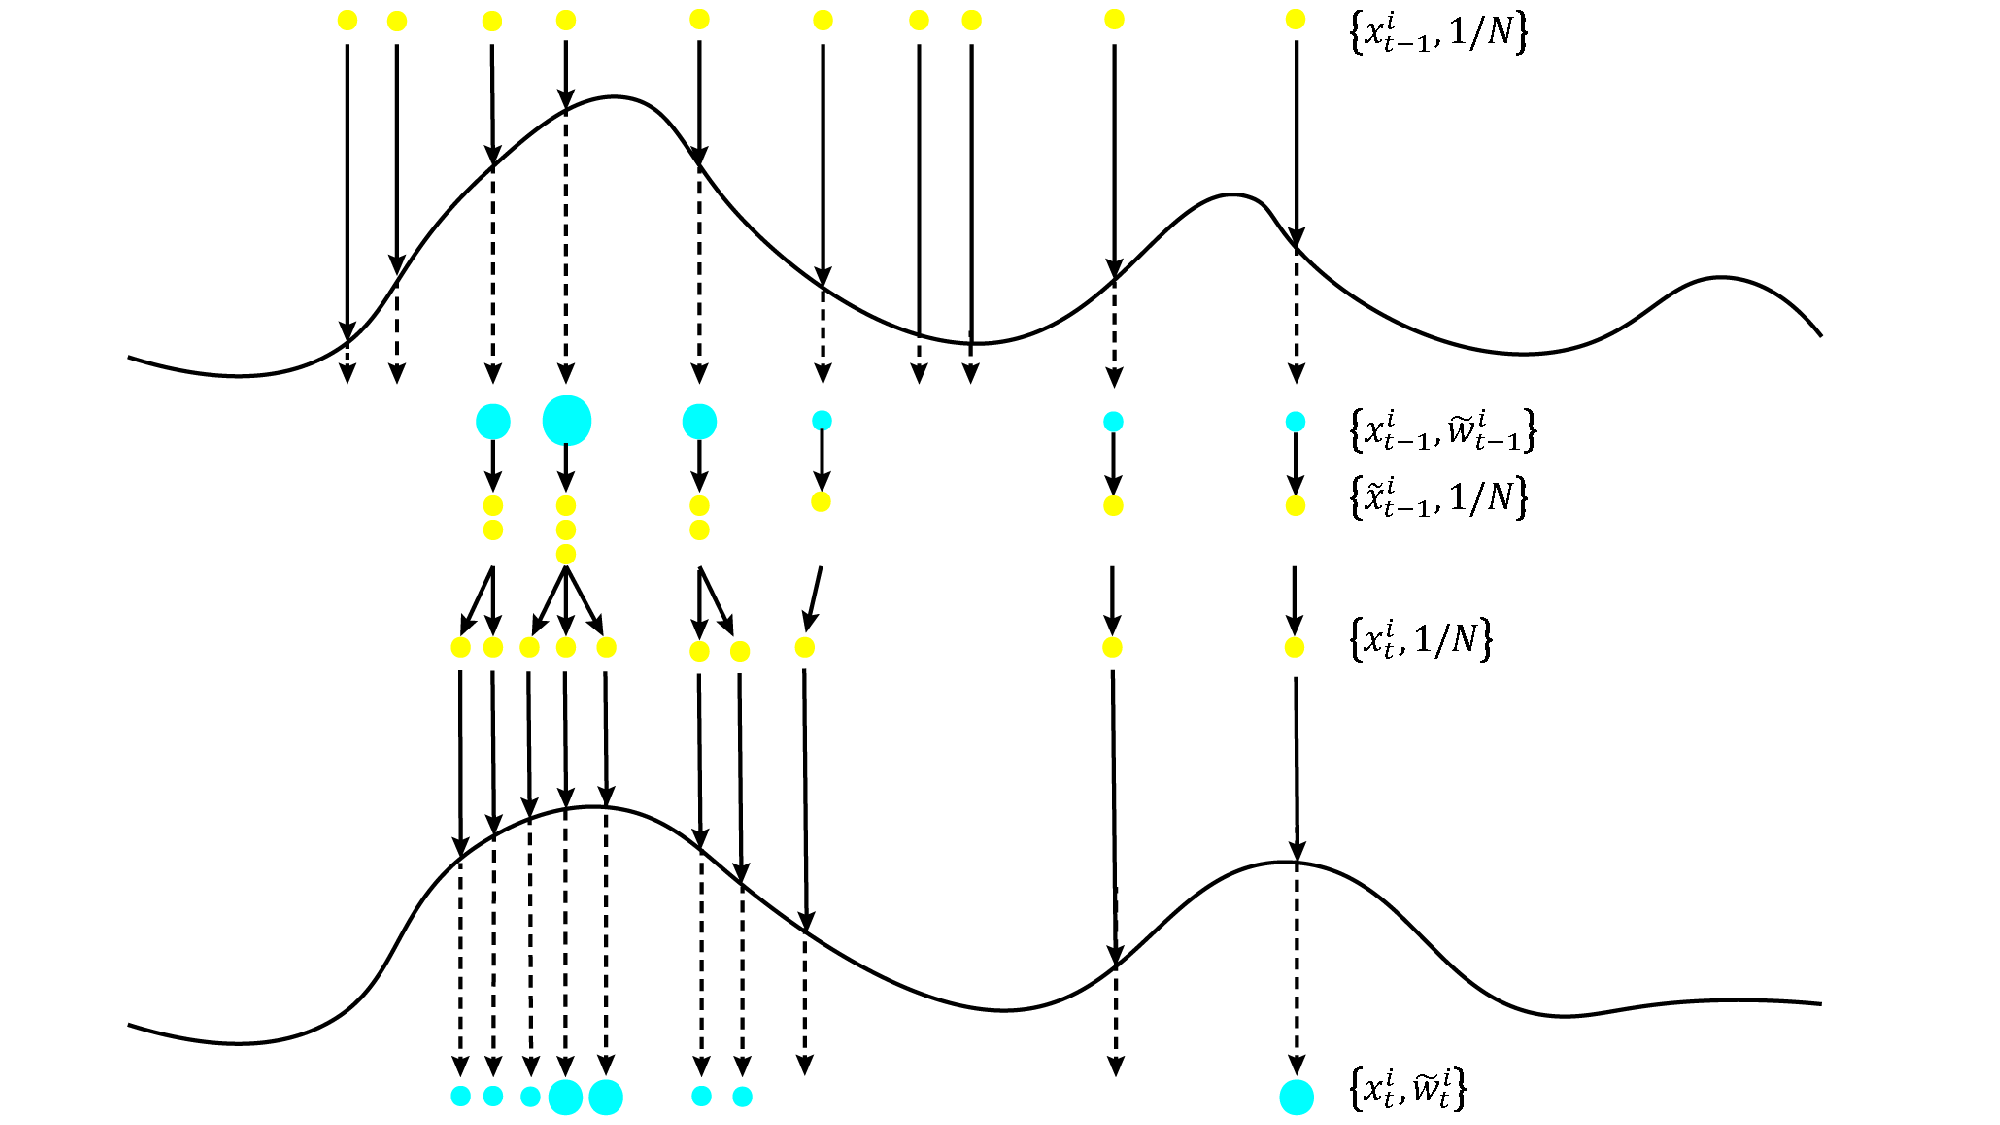
\includegraphics[width=1.0\linewidth]{PF_figure.pdf}
    \caption{Particle Filter Process.}
    \label{fig:pf}
\end{figure}

\noindent Since we can estimate the posterior probability density and posterior state by particle filter now,
the corresponding likelihood (\ref{likelihood}) then can also be approximated.
For estimating the likelihood, we introduce the auxiliary particle filter(APF) algorithm developed
from the above standard PF algorithm.
The APF is a popular approach covering as special cases a large class of particle algorithms, such as the bootstrap filter.\\

\noindent Given
the particles at time $t-1$, the APF proceeds to time $t$  by three steps.\\
\begin{enumerate}
    \item Resampling: The particles are resampled according to their auxiliary weights.
    The result is an equally-weighted particle
    system $\left\{\tilde{x}_{t}^{(i)}, 1/N ; i=1,2, \cdots, N\right\}$.\\
    
    \item Propagation: The particles are propagated to time $t$ by sampling from a proposal kernel
    $x_{t}^{(i)} \sim R_{\theta}\left(x_{t} \mid \widetilde{x}_{t-1}^{(i)}, y_{t}\right)$.\\
    
    \item Weighting: The (unnormalised) particle weight is calculated for each particle. The importance weights are given by
    \begin{equation}w_{t}^{(i)}=W_{\theta}\left(x_{t}^{(i)}, \tilde{x}_{t-1}^{(i)}\right)=\frac{g_{\theta}\left(y_{t} \mid x_{t}^{(i)}\right) f_{\theta}\left(x_{t}^{(i)} \mid \widetilde{x}_{t-1}^{(i)}\right)}{R_{\theta}\left(x_{t}^{(i)} \mid \widetilde{x}_{t-1}^{(i)}, y_{t}\right)}.\end{equation}
    The bootstrap PF is just a special case of APF when
    $R_{\theta}\left(x_{t}^{(i)} \mid \widetilde{x}_{t-1}^{(i)},y_{t}\right)=f_{\theta}\left(x_{t}^{(i)} \mid \widetilde{x}_{t-1}^{(i)}\right)$, and thus $w_{t}^{(i)}=g_{\theta}\left(y_{t} \mid x_{t}^{(i)}\right)$. More sophisticated alternatives of
    $R_{\theta}$ exist, for example, the fully-adapted PF.
\end{enumerate}

\noindent Then we can calculate equation (\ref{y}) by \\
\begin{equation}\begin{aligned}
    p_{\theta}\left(y_{t} \mid y_{1: t-1}\right)&=
    \int p_{\theta}\left(x_{1:t-1} \mid y_{1:t-1}\right)
    p_{\theta}\left(x_{t} \mid x_{t-1}\right) p_{\theta}\left(y_{t} \mid x_{t}\right) \mathrm{d} x_{1:t}\\
    &=
   \int p_{\theta}\left(x_{t-1} \mid y_{1: t-1}\right)p_{\theta}\left(x_{t} \mid x_{t-1}\right) p_{\theta}\left(y_{t} \mid x_{t}\right) \mathrm{d} x_{t-1: t} \\
   &=\int W_{\theta}\left(x_{t}, x_{t-1}\right) R_{\theta}\left(x_{t} \mid x_{t-1}, y_{t}\right) p_{\theta}\left(x_{t-1} \mid y_{1: t-1}\right) \mathrm{d} x_{t-1: t}.
\end{aligned}\end{equation}\\

\noindent To approximate the integral, we note that
the (unweighted) particle pairs $\left\{\widetilde{x}_{t-1}^{(i)}, x_{t}^{(i)}\right\}_{i=1}^{N}$ are approximately
drawn from $R_{\theta}\left(x_{t} \mid x_{t-1}, y_{t}\right) p_{\theta}\left(x_{t-1} \mid y_{1: t-1}\right)$.
Consequently,
 the MC approximation of the above equation is obtained by
\begin{equation}p_{\theta}\left(y_{t} \mid y_{1: t-1}\right) \approx \frac{1}{N} \sum_{i=1}^{N} w_{t}^{(i)}.\end{equation}
\noindent By inserting this approximation into equation (\ref{likelihood}),  we obtain the
particle estimate of the likelihood
\begin{equation}\widehat{\mathcal{L}}(\theta)=\prod_{t=1}^{T}\left(\frac{1}{N} \sum_{i=1}^{N} w_{t}^{(i)}\right).\end{equation}\\
\noindent However, working directly with the likelihood typically
results in numerical difficulties. To avoid this problem in practice, we instead use an estimate of the log-likelihood
\begin{equation}\widehat{\ell}(\theta)=\log \widehat{\mathcal{L}}(\theta)=\sum_{t=1}^{T} \log \left[\sum_{i=1}^{N} w_{t}^{(i)}\right]-T \log N.\end{equation}

\noindent The algorithm for approximating the likelihood(log-likelihood) can thus be summarised as follows.\\


\begin{algorithm} [H] 
\caption{APF for log-likelihood estimation}  
\hspace*{0.02in}{\bf Input:}
An SSM, observations: $y_{1:T}$, no. particles: $N$.\\
\hspace*{0.02in}{\bf Output:} 
 MC estimation of the log-likelihood: $\widehat{\ell}(\theta)$.

\begin{algorithmic}[1] 
\STATE {Initialise particles $x_{1}^{(i)}$for $i=1$
to $N$.}
\STATE{for $t = 1$ to $T$ do}
\STATE{\quad Resample the particles with weights $\left\{w_{t-1}^{(i)}\right\}_{i=1}^{N}$.} 
\STATE{\quad Propagate the particles using $R_{\theta}\left(\cdot\right)$.}
\STATE{\quad Calculate new importance weights $\left\{w_{t}^{(i)}\right\}_{i=1}^{N}$.}
\STATE{end for}
\STATE{Compute log-likelihood $\widehat\ell(\theta) $.}
\end{algorithmic}  
\end{algorithm}

\noindent As previously discussed, the likelihood $\mathcal{L}(\theta)$ and log-likelihood $\ell(\theta)$ play important
roles in both ML and Bayesian parameter inference.
Details relating to
parameter inference  will be discussed in the next chapter. \\


\noindent In practice, any physical system is nonlinear,
as long as it is analyzed with sufficient precision.
Therefore, PF algorithms are developing rapidly in various fields because of the good  estimation performance in nonlinear and non-Gaussian systems.\\

\section{State Estimation in  Linear Gaussian SSM}
In this section, we start to implement the PF algorithm based on the process we discussed in the previous sections. To simplify, we consider the basic linear Gaussian state-space (LGSS) model.\\

\noindent The particular LGSS model considered is given by
\begin{equation}\label{lgss}
x_{1} \sim \mu_{\theta}\left(x_{1}\right), \quad x_{t}\left|x_{t-1} \sim \mathcal{N}\left(x_{t} ; \phi x_{t-1}, \sigma_{v}^{2}\right), \quad y_{t}\right| x_{t} \sim \mathcal{N}\left(y_{t} ; x_{t}, \sigma_{e}^{2}\right),\end{equation}
where parameters are denoted by
$\theta=\left\{\phi, \sigma_{v}, \sigma_{e}\right\}$
and $\mathcal{N}\left(x ; \mu, \sigma^{2}\right)$
denote the Gaussian density with
mean $\mu$ and standard deviation $\sigma > 0$.
$\phi \in(-1,1)$ determines the persistence
of the state, while $\sigma_{v}, \sigma_{e} \in \mathbb{R}_{+}$ denote the standard deviations of the state transition noise
and the observation noise, respectively.\\

\noindent We begin with generating data from the
model with $T=250$ observations and $\theta =\left\{0.75,1.00,0.10\right\}, x_{1}=0$. Figure \ref{fig:datagene}
shows the simulated data record.\\
\begin{figure}[H]
    \centering
    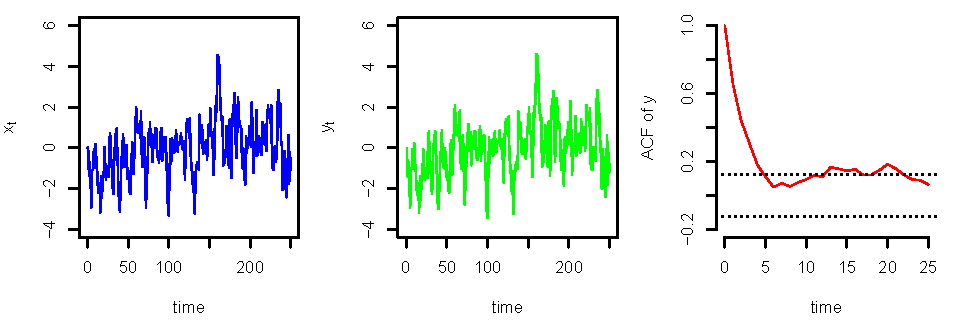
\includegraphics[width=1.0\linewidth]{datagene.pdf}
    \caption
    {Simulated data from the LGSS model with latent state (left), observations (middle), and autocorrelation function (ACF) of the observations (right).}
    \label{fig:datagene}
\end{figure}

\noindent Then we make use of the implementation of particle filter algorithm to estimate the filtered state and
to investigate the properties of this estimate. The estimates from the particle filter are
compared with the corresponding estimates from the Kalman filter. As we have discussed in the previous
sections, KF  algorithm  is   an  optimal  filtering algorithm for LGSS model. Thus, comparing with Kalman filter
is a sensible way to measure the performance of particle filter algorithm. \\

\noindent On the top of Figure \ref{fig:state}, is the set of observations simulated from the LGSS model we mentioned before. In the middle  we present the difference between the  state estimate from
the Kalman filter and the estimate from the particle filter algorithm using N = 2000 particles.
The accuracy of particle filter algorithm can also be measured by
the bias (absolute error) and the mean square error
(MSE) of the state estimation.
The bias is defined by 
\begin{equation}\operatorname{Bias}\left(\widehat{x}_{t}^{N}\right)=\frac{1}{T} \sum_{t=1}^{T}\left|\widehat{x}_{t}^{N}-\widehat{x}_{t}\right|,\end{equation}
and the mean square error is denoted by
\begin{equation}\operatorname{MSE}\left(\widehat{x}_{t}^{N}\right)=\frac{1}{T} \sum_{t=1}^{T}\left(\widehat{x}_{t}^{N}-\widehat{x}_{t}\right)^{2},\end{equation}
where $\widehat{x}_{t}^{N}$ denotes the estimation from
PF algorithm and $\widehat{x}_{t}$ is the estimation obtained by KF algorithm. Their logarithms for different
values of $N$ are presented in the bottom of  Figure \ref{fig:state}. We can see that the bias and the MSE decrease rapidly as N increases.\\

\begin{figure}[H]
    \centering
    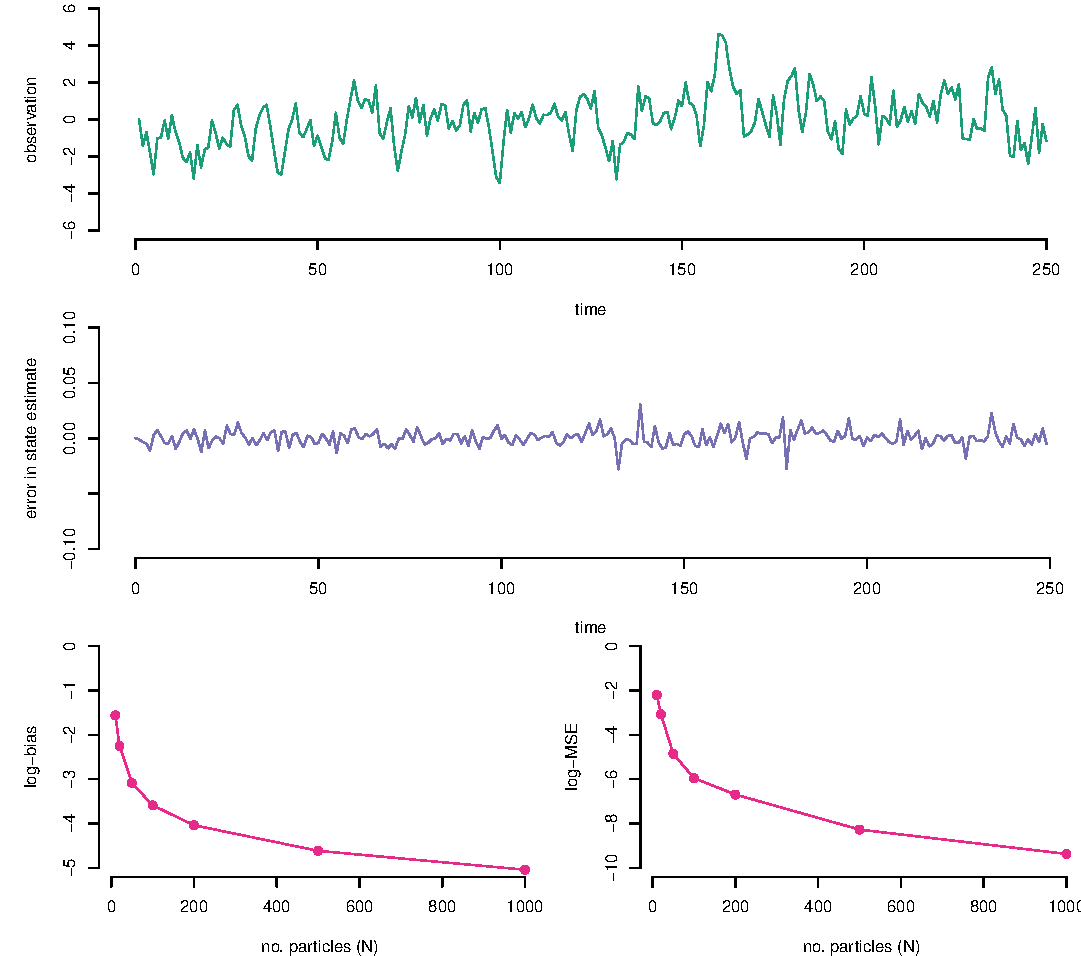
\includegraphics[width=1.0\linewidth]{state.pdf}
    \caption
    {Top: a simulated set of observations $y_{t}$ from the LGSS model. Middle: the error in latent state  estimate using  particle filter algorithm with
    N = 2000. Bottom: the
    estimated log-bias (left) and log-MSE (right) for the particle filter algorithm with different number
    of particles N.}
    \label{fig:state}
\end{figure}











%%%%%%%%%%%%


\chapter{Parameter Inference
Using Particle Methods}
In this chapter, We describe how the particle filtering
algorithm can be used to implement
parameter inference techniques.
We give some overview of Bayesian parameter inference
and  maximum likelihood parameter inference first
and then proceeds with the implementation of these methods with some examples.



\section{Bayesian parameter inference}
\subsection{Overview of Bayesian methods }
Sampling based approaches  or approximate
analytical computations are main ideas to do Bayesian parameter inference.
Examples of sampling based approaches are MCMC methods or SMC methods \cite{chopin2013smc2}.
Examples of analytical approximations are the integrated nested Laplace approximation (INLA) \cite{rue2009approximate}, variational Bayes (VB) \cite{bishop2006pattern},
and expectation propagation (EP) \cite{minka2013expectation}.\\

\noindent In this section, we are primarily interested in
 the particle Metropolis-Hastings
(PMH) algorithm for Bayesian parameter inference and some examples will be shown here. A tutorial article \cite{dahlin2019getting}  provides a comprehensive introduction to the particle Metropolis-Hastings (PMH) algorithm for parameter inference. We do not introduce the details about PMH in this thesis.
We just do parameter inference by PMH method mentioned in 
that tutorial article first in this section and
then compare with the results from ML methods in next section.\\

\subsection{Estimating the parameters in LGSS model}\label{section_lgss_inference}
To simplify the parameter inference problem in the LGSS model (\ref{lgss}), we assume $\theta=\phi$ is the only unknown parameter and keep $\left\{\sigma_{v}, \sigma_{e}\right\}=\left\{1.00,0.10\right\}$ fixed to
their true values. Following the PMH algorithm in article \cite{dahlin2019getting},  setting the initial value of
the Markov chain by $\theta_{0}=0.5$,  the number of iterations by $K=2000$, and the number of particles by $N=5000$, we can get the results of parameter inference by PMH algorithm as shown in 
figure \ref{fig:mph_lgss}.
Three runs of PMH are presented using different step sizes $\epsilon$ = 0.01 (left), 0.10
(center) and 0.50 (right).
To make sure that the Markov chain  has reached its stationary regime,
we discard the first 1000 iterations as burn-in and only use the
last 1000 iterations to approximate the parameter
posterior.\\

\noindent The resulting estimate of the posterior mean is
$\widehat{\phi}=0.66$ for $\epsilon=0.01$ and 0.1, and 
$\widehat{\phi}=0.65$ for $\epsilon=0.5$. Actually, the choice of $\epsilon$ influences the correlation
in the Markov chain, thus a good choice of $\epsilon$ is important to obtain an efficient algorithm. 
We note that the 
posterior estimate of unknown parameter differs slightly from the true value 0.75. From the asymptotic theory of the Bayesian estimator, we know that this is due to the
relatively small sample size $T$ and a finite $K$. If we 
set number of observations $T= 500$, we will get the result
$\widehat{\phi}=0.72$, which is much closer to the true value
0.75. And also, the estimated posterior variance will be smaller, which means the results are more stable when $T$ goes larger.



\begin{figure}[H]
    \centering
    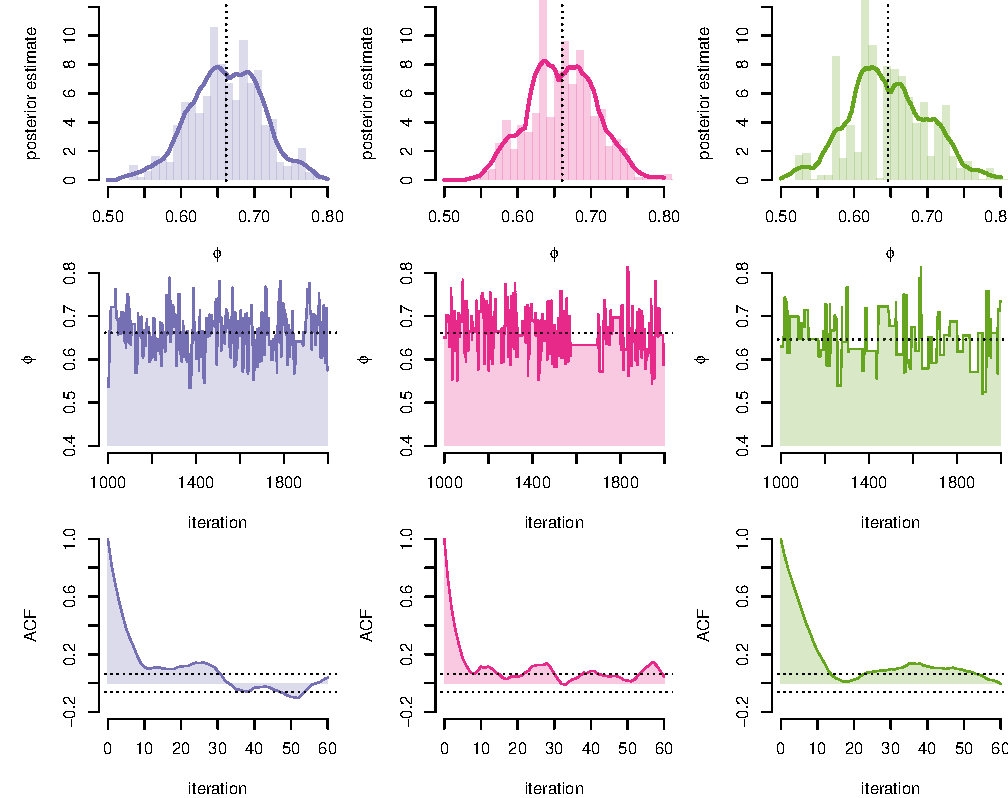
\includegraphics[width=1.0\linewidth]{MyExample2.pdf}
    \caption
    {The parameter inference results using PMH methods for different step  sizes:$\epsilon$ = 0.01 (left), 0.10
    (center) and 0.50 (right). Top: histogram and kernel density estimate.
    Middle: the state of
    the Markov chain after the 1000 burn-in. 
    Bottom: the estimated ACF of the
    Markov chain.
    Dotted lines in the top and middle plots indicate
    mean value and the dotted lines in the bottom plot indicate the $95\%$ confidence intervals of the ACF
    coefficients.}
    \label{fig:mph_lgss}
\end{figure}

\subsection{Estimating the parameters in nonlinear model}
We now  proceeds with application of the PMH algorithm to infer the parameters of a nonlinear SSM called stochastic volatility model \cite{hull1987pricing}. 
The  SV model is defined  by
\begin{equation}\label{sv_model}
\begin{aligned}
x_{1} & \sim \mathcal{N}\left(x_{1} ; \mu, \frac{\sigma_{v}^{2}}{1-\phi^{2}}\right), \\
x_{t+1} \mid x_{t} & \sim \mathcal{N}\left(x_{t+1} ; \mu+\phi\left(x_{t}-\mu\right), \sigma_{v}^{2}\right), \\
y_{t} \mid x_{t} & \sim \mathcal{N}\left(y_{t} ; 0, \exp \left(x_{t}\right)\right),
\end{aligned}\end{equation}
where the parameters are denoted by $\theta=\left\{\mu, \phi, \sigma_{v}\right\}$. Here, $\mu \in \mathbb{R}, \phi \in[-1,1]$ and $\sigma_{v} \in  \mathbb{R}_{+}$
denote the mean value, the persistence and standard deviation of the state process,
respectively.\\

\noindent This model is important in econometrics, where  the latent state $x_{t}$ is known as the log-volatility and the observations $y_{t}$ are so-called log-returns. The log-volatility is useful for risk management and to price various financial contracts \cite{hull2009options}.\\

\noindent In the tutorial article \cite{dahlin2019getting},
the data
from Quandl for the period between January 2, 2012 and January 2, 2014 are extracted to do parameter inference
and the  resulting estimate are shown in Figure \ref{fig:svpmh}.

\begin{figure}[H]
    \centering
    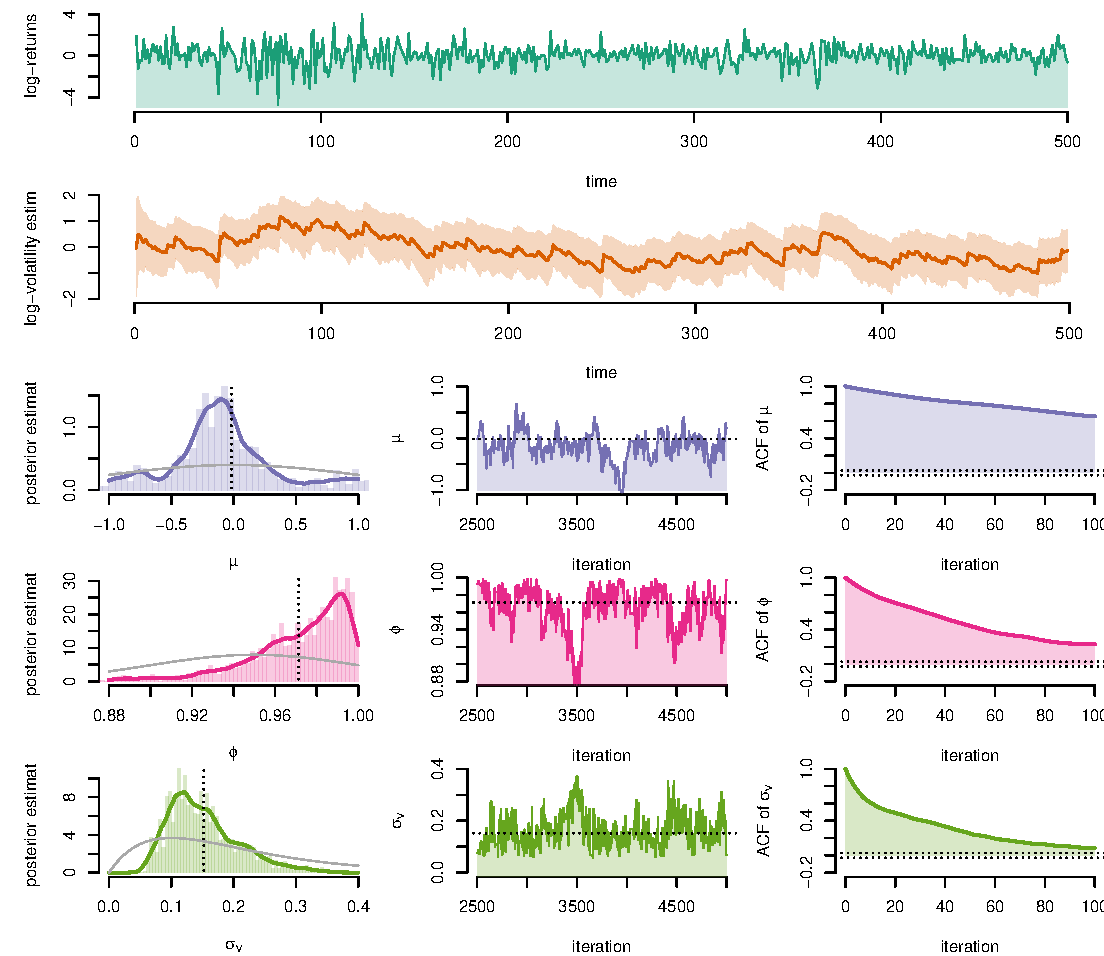
\includegraphics[width=1.0\linewidth]{svpmh.pdf}
    \caption
    {First two lines: the daily log-returns and estimated log-volatility  with
    $95\%$ confidence intervals of the NASDAQ OMXS30 index for the period between January 2,
    2012 and January 2, 2014.
    Bottom: the posterior estimate (left), the trace of the Markov
    chain (middle) and the corresponding ACF (right) of the parameters obtained from PMH.}
    \label{fig:svpmh}
\end{figure}



\section{Maximum likelihood parameter inference}
\subsection{Overview of ML methods }
The parameter inference problem in the ML framework is
described in equation (\ref{ML}). In most situations,
it cannot be solved by
analytical calculations. Instead popular approaches are mainly based on optimisation and
other iterative algorithms.
Gradient-based optimisation
algorithms \cite{poyiadjis2011particle,yildirim2015parameter} are widely used to maximise the log-likelihood and thereby estimate the parameters of
the model. This method operates by an iterative application of
\begin{equation}\widehat{\theta}_{k+1}=\widehat{\theta}_{k}+\epsilon_{k} \widehat{\mathcal{S}}\left(\theta_{k}\right).\end{equation}
where $\widehat{\theta}_{k}$ denotes the current estimate of the parameter vector and $\widehat{\theta}_{k+1}$ is the proposed next estimate. 
$\epsilon_{k}$ means the step length and $\widehat{\mathcal{S}}\left(\theta_{k}\right)$ is the score function which we will discuss in detail and show how to calculate later.
Furthermore, if we can estimate the Hessian matrix,
Newton optimisation algorithm can be implemented by
iteration of
\begin{equation}\label{Newton}
\widehat{\theta}_{k+1}=\widehat{\theta}_{k}+\epsilon_{k} \widehat{\mathcal{J}}^{-1}\left(\theta_{k}\right) \widehat{\mathcal{S}}\left(\theta_{k}\right).\end{equation}
where $\widehat{\mathcal{J}}$ is the information matrix (negative Hessian).\\

\noindent Another popular method for ML inference
is the expectation maximisation algorithm where
the latent states are seen as missing information and are estimated together with
the parameter vector of the model. An additive functional
which can be obtained by smoothing is required in this algorithm. 
By using different smoothing method, we can obtain different kinds of expectation maximisation algorithm   
\cite{del2010forward,lindsten2013backward,schon2011system}.\\


\noindent Here we are mainly interested in the Newton optimisation algorithm. Before we implement the algorithm, from equation
(\ref{Newton}) we know that we should first calculate the score function and the observed information
matrix by particle filter algorithm.\\

\noindent Fisher’s identity for the score vector of the log-likelihood is
\begin{equation}\label{score}
\nabla \log p_{\theta}\left(y_{1: t}\right)=\int \nabla \log p_{\theta}\left(x_{1: t}, y_{1: t}\right) p_{\theta}\left(x_{1: t} \mid y_{1: t}\right) d x_{1: t}.\end{equation}
Similarly, the observed information matrix satisfies Louis’ identity
\begin{equation}-\nabla^{2} \log p_{\theta}\left(y_{1: t}\right)=\nabla \log p_{\theta}\left(y_{1: t}\right) \nabla \log p_{\theta}\left(y_{1: t}\right)^{\mathrm{T}}-\frac{\nabla^{2} p_{\theta}\left(y_{1: t}\right)}{p_{\theta}\left(y_{1: t}\right)},\end{equation}
where
\begin{equation}\label{info}
\begin{aligned}
\frac{\nabla^{2} p_{\theta}\left(y_{1: t}\right)}{p_{\theta}\left(y_{1: t}\right)}=& \int \nabla \log p_{\theta}\left(x_{1: t}, y_{1: t}\right) \nabla \log p_{\theta}\left(x_{1: t}, y_{1: t}\right)^{\mathrm{T}} p_{\theta}\left(x_{1: t} \mid y_{1: t}\right) d x_{1: t} \\
&+\int \nabla^{2} \log p_{\theta}\left(x_{1: t}, y_{1: t}\right) p_{\theta}\left(x_{1: t} \mid y_{1: t}\right) d x_{1: t}.
\end{aligned}\end{equation}\\

\noindent To recursively compute the score and observed information matrix, we define the vector $\alpha_{t}^{(i)}=\nabla \log p_{\theta}\left(x_{1: t}^{(i)}, y_{1: t}\right)$, and the matrix $\beta_{t}^{(i)}=\nabla^{2} \log p_{\theta}\left(x_{1: t}^{(i)}, y_{1: t}\right)$. Then the particle approximation process for score vector and information matrix proceeds as follows.\\

\begin{enumerate}
    \item Resample the particle set $\left\{x_{1: t-1}^{(i)}, \alpha_{t-1}^{(i)}, \beta_{t-1}^{(i)}\right\}_{i=1}^{N}$ using the weights
    $\left\{w_{t-1}^{(i)}\right\}$ to obtain a set of N new particles.
    \item For $i =1, \cdots , N$, sample $x_{t}^{(i)} \sim q_{\theta}\left(\cdot \mid y_{t}, x_{t-1}^{(i)}\right)$, and compute the weights
    \begin{equation}w_{t}^{(i)} \propto \frac{g_{\theta}\left(y_{t} \mid x_{t}^{(i)}\right) f_{\theta}\left(x_{t}^{(i)} \mid x_{t-1}^{(i)}\right)}{q_{\theta}\left(x_{t}^{(i)}, y_{t} \mid x_{t-1}^{(i)}\right)}.\end{equation}
    \item Update $\left\{\alpha_{t}^{(i)}, \beta_{t}^{(i)}\right\}_{i=1}^{N}$, the score estimate $S_{t}$ and observed information matrix estimate $\Sigma_{t}$:
    \begin{equation}\begin{aligned}
\alpha_{t}^{(i)} &=\alpha_{t-1}^{(i)}+\nabla \log g_{\theta}\left(y_{t} \mid x_{t}^{(i)}\right)+\nabla \log f_{\theta}\left(x_{t}^{(i)} \mid x_{t-1}^{(i)}\right) \\
\beta_{t}^{(i)} &=\beta_{t-1}^{(i)}+\nabla^{2} \log g_{\theta}\left(y_{t} \mid x_{t}^{(i)}\right)+\nabla^{2} \log f_{\theta}\left(x_{t}^{(i)} \mid x_{n-1}^{(i)}\right) \\
S_{t} &=\sum_{i=1}^{N} w_{t}^{(i)} \alpha_{t}^{(i)}, \quad \text { and } \quad \Sigma_{t}=S_{t} S_{t}^{\mathrm{T}}-\sum_{i=1}^{N} w_{t}^{(i)}\left(\alpha_{t}^{(i)} \alpha_{t}^{(i) \mathrm{T}}+\beta_{t}^{(i)}\right).
\end{aligned}\end{equation}
\end{enumerate}
The estimates are obtained by  substituting $\hat{p}_{\theta}\left(x_{1:t} \mid y_{1: t}\right)$ for $p_{\theta}\left(x_{1:t} \mid y_{1: t}\right)$ into equations
(\ref{score}) - (\ref{info}).\\

\subsection{Estimating the parameters in LGSS model}
Consider the LGSS model (\ref{lgss}) with the true parameter vector $\theta^{*}=\left\{0.75,1.00,0.10\right\}$.
We generate data of length $T = 500$ using the initial value $x_{1} = 0$. As assumed in section \ref{section_lgss_inference}, here $\phi$ is chosen to be the single unknown parameter and 
$\left\{\sigma_{v}, \sigma_{e}\right\}=\left\{1.00,0.10\right\}$ fixed to
their true values.
We set the  number  of  particles  by $N=  5000$ and calculate the log-likelihood, the score function and the expected information
matrix for different value of $\phi$.
The results are presented in Figure \ref{fig:score_lgss}.\\

\noindent It can be seen obviously in the figure that the  maximum of the log-likelihood is near the true parameter
and  the score function is zero close to
this point.
Since the score function is the slope of the log-likelihood,
the zero of the score function results in a maximum of the
log-likelihood function when the expected information (negative Hessian) is positive.

\begin{figure}[H]
    \centering
    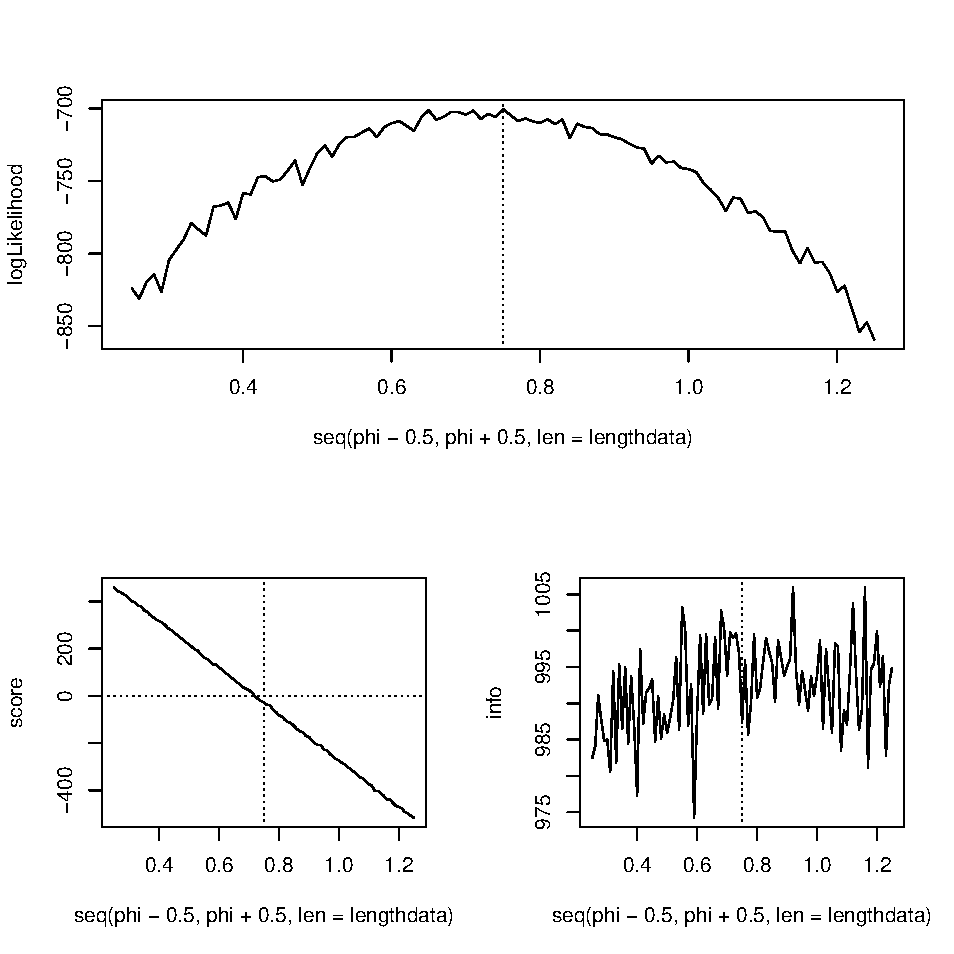
\includegraphics[width=1.0\linewidth]{score_lgss.pdf}
    \caption
    {The estimates of the log-likelihood (top) the score
    function (bottom left) and the expected information matrix (bottom right) of the
    LGSS model by PF algorithm. The dotted lines indicate the true value of the parameter $\phi$ (0.75).}
    \label{fig:score_lgss}
\end{figure}

\noindent Now that we have the estimates of log-likelihood, score function and expected information, we can infer the value of $\phi$ by Newton optimisation.
Here we set a stopping point $\lvert\widehat{\theta}_{k+1}-\widehat{\theta}_{k} < 0.001 \rvert$  and initial value $\theta_{1}=0.5$ for the iteration equation (\ref{Newton}).
That is, when this condition is arrived, we stop the iteration and return $\widehat{\theta}_{k+1}$ as our estimate for the parameter. This method converges much fater than the PMH method  and the iteration will often be stopped in ten times.  
However, in the PMH algorithm, we should discard the first 1000 iterations to ensure the stability.\\

\noindent To get a more convincing results, we generate 500 data sets from the same true parameter vector and then run the estimation procedure on each of the simulated data set to get 500 estimated parameter vectors. The results are presented in Figure \ref{fig:500test}. The mean value of the 500 estimated parameter is $\widehat{\phi}=0.746$ with standard deviation
= 0.03, which is very close to the true value 0.75. What's more, if we change the initial value of the iteration, both the convergence rate and the estimated results are consistent(almost no difference).
Therefore, it seems that Newton optimisation based on
PF algorithm is an efficient way to do parameter inference in SSMs.

\begin{figure}[H]
    \centering
    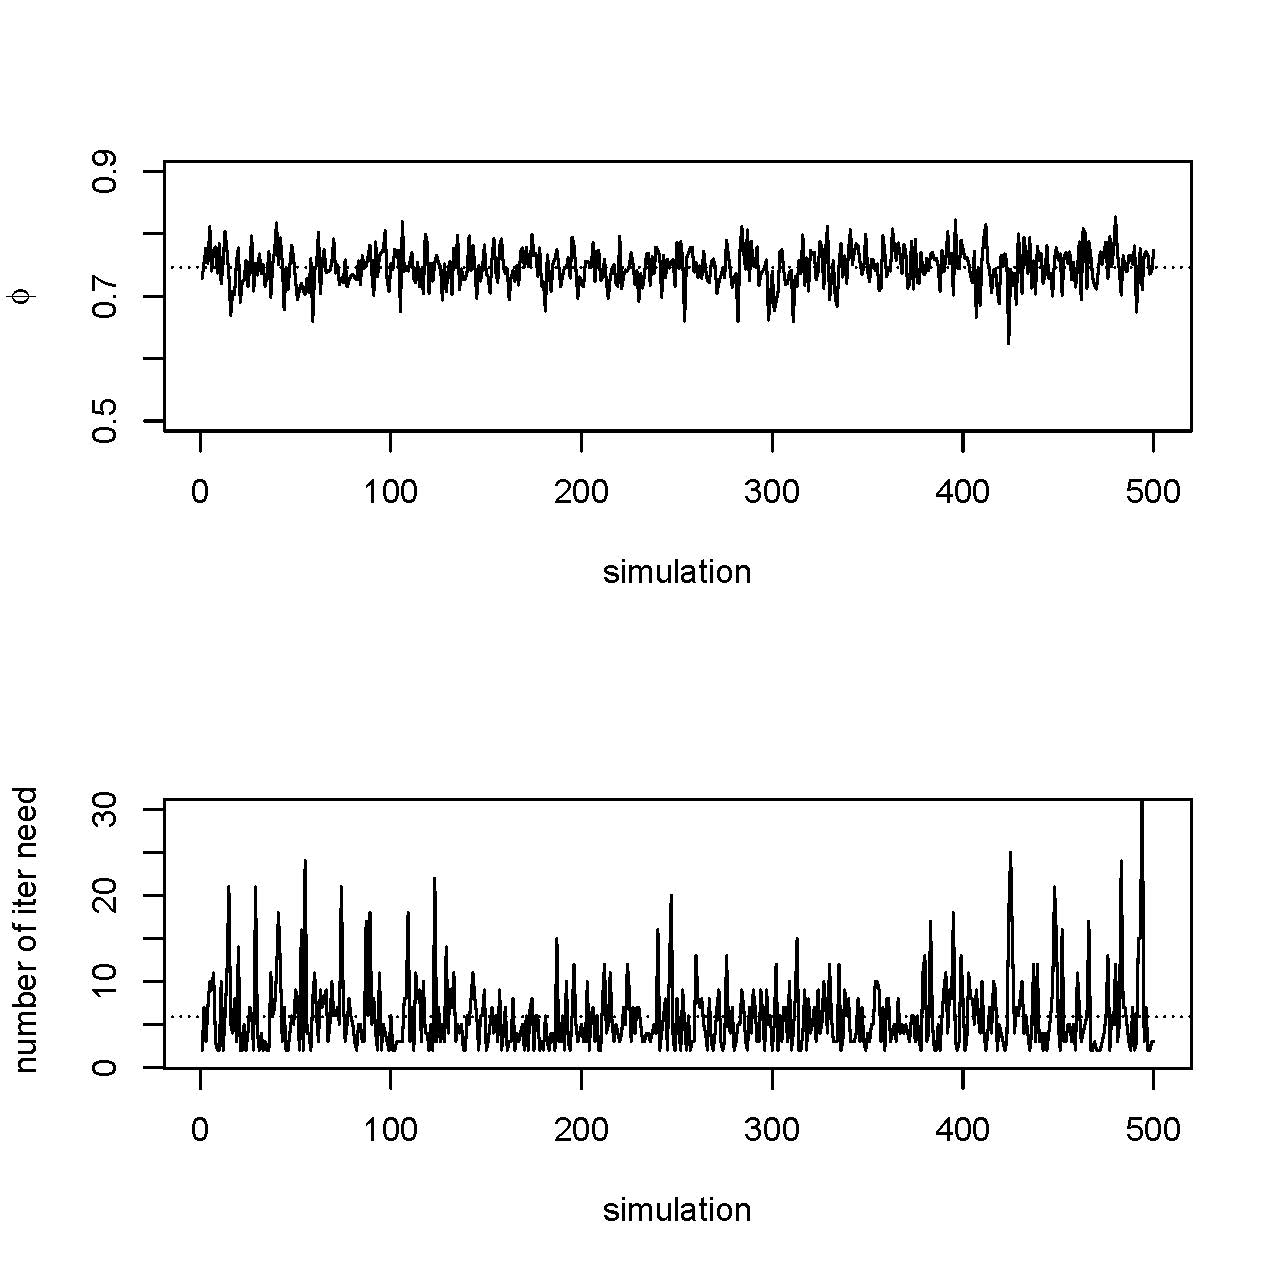
\includegraphics[width=1.0\linewidth]{500test.jpg}
    \caption
    {Estimated results by Newton optimisation. Top: estimated value of parameter. Bottom:  number of iterations to converge. The dotted lines are the mean value of 500 simulations.}
    \label{fig:500test}
\end{figure}


\subsection{Estimating the parameters in nonlinear model}
Similarly, to work on the SV model defined by equation (\ref{sv_model}),
we generate  data of length $T=1000$ with true parameter vector 
$\theta^{*}=\left\{\mu^{*}, \phi^{*}, \sigma_{v}^{*}\right\}
=\left\{-1.02,0.95,0.25\right\}$.\\

\noindent If we choose $\phi$ to be the unknown parameter, the estimates
of the log-likelihood, the score function and the expected information
are presented in Figure \ref{fig:score_phi}. Similar to the results of the LGSS model, at the position close to the true value of the parameter, the  log-likelihood
has a maximum, the score function is zero and the expected information is positive.

\begin{figure}[H]
    \centering
    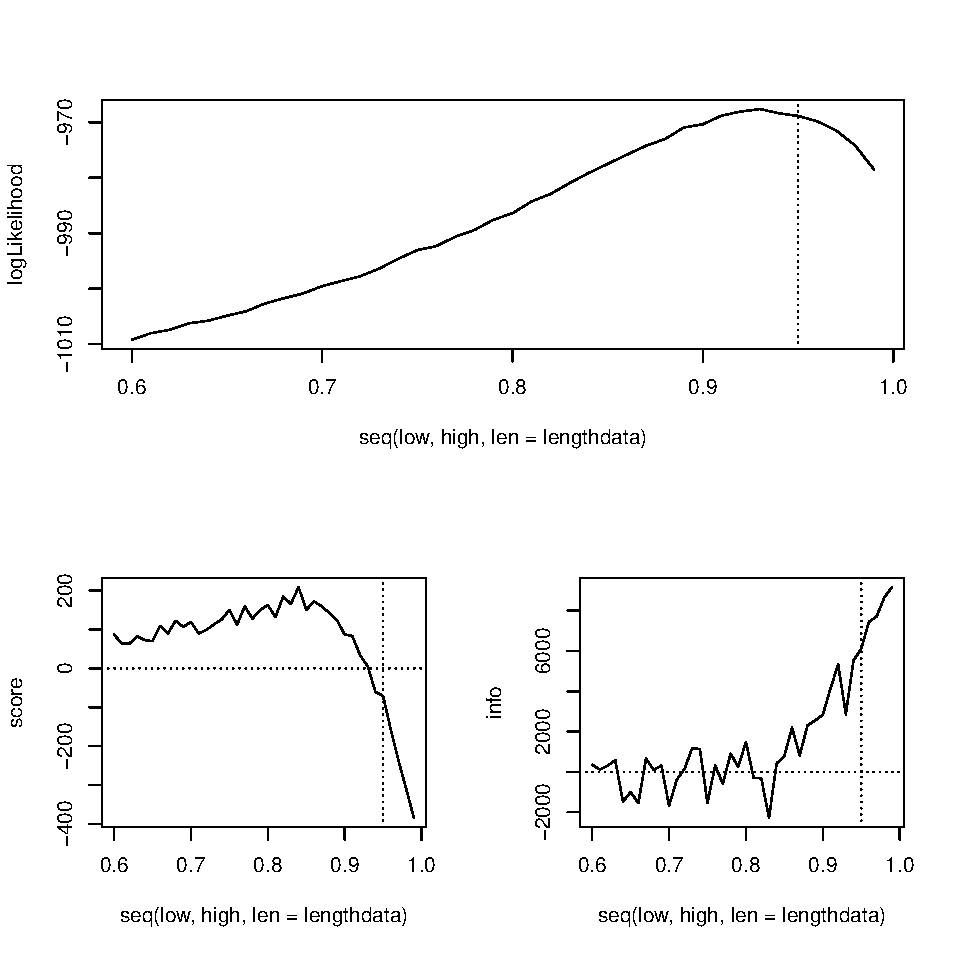
\includegraphics[width=1.0\linewidth]{score_phi.pdf}
    \caption
    {The estimates of the log-likelihood (top) the score
    function (bottom left) and the expected information matrix (bottom right) of the
    SV model by PF algorithm for different values of $\phi$. The dotted lines indicate the true value of the parameter $\phi$ (0.95).}
    \label{fig:score_phi}
\end{figure}

\noindent  The estimates based on choosing $\mu$ to be the unknown parameter also returns the same results, see Figure \ref{fig:score_mu}.
We note that the curve of log-likelihood  here is not as smooth as other examples we mentioned before. We can make it smooth by choosing a larger value of $T$.

\begin{figure}[H]
    \centering
    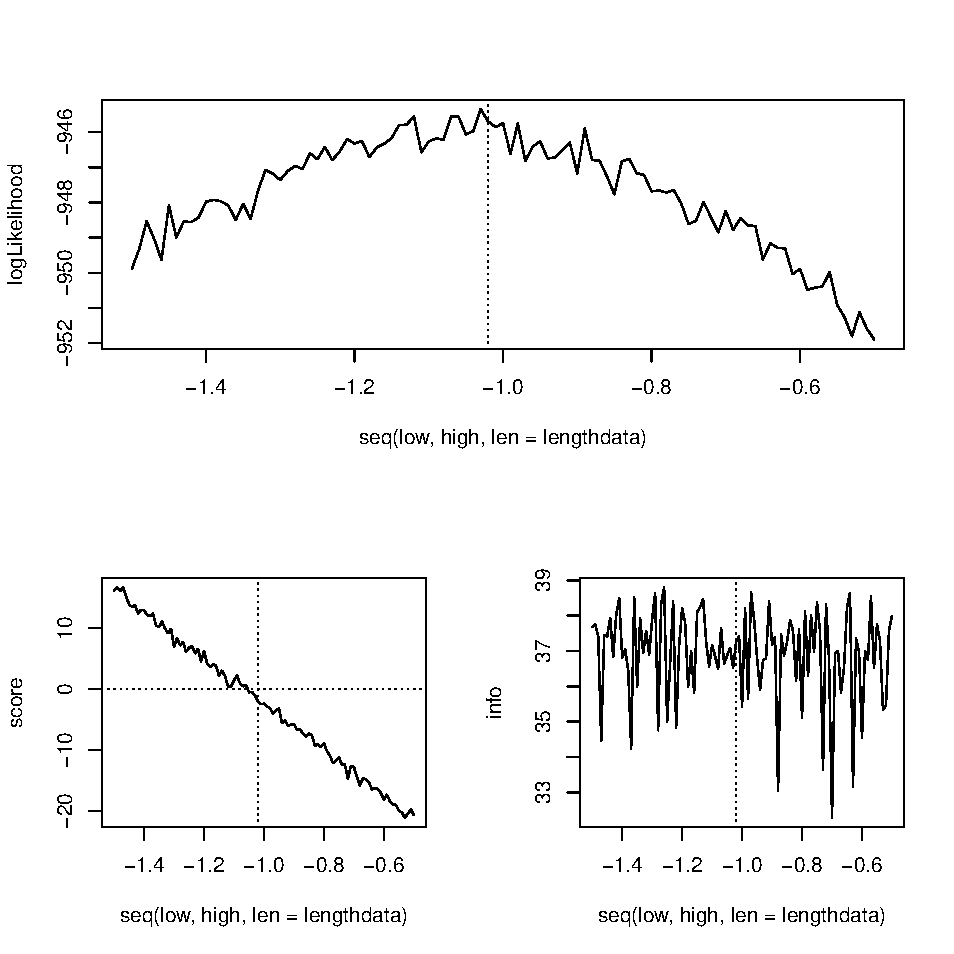
\includegraphics[width=1.0\linewidth]{score_mu.pdf}
    \caption
    {The estimates of the log-likelihood (top) the score
    function (bottom left) and the expected information matrix (bottom right) of the
    SV model by PF algorithm for different values of $\mu$. The dotted lines indicate the true value of the parameter $\mu$ (-1.02).}
    \label{fig:score_mu}
\end{figure}


\noindent Then we simulate 500 data set to infer the parameter.
Results for $\phi$ and $\mu$ are presented in Figure \ref{fig:scoremethod_phi} and Figure \ref{fig:scoremethod_mu} respectively.
The mean value of the estimated parameter is $\widehat{\phi}=0.9495$, with $95\%$ confidence interval [0.9339, 0.9652] and $\widehat{\mu}=-1.0254$, with $95\%$ confidence interval [-1.3505, -0.7004].
We note that for both $\phi$ and $\mu$, the Newton  optimisation based on particle filter method gives a good resulting estimate of the true value. Compared with the PMH algorithm, Newton  optimisation convergences much faster and returns more accurate results.


\begin{figure}[H]
    \centering
    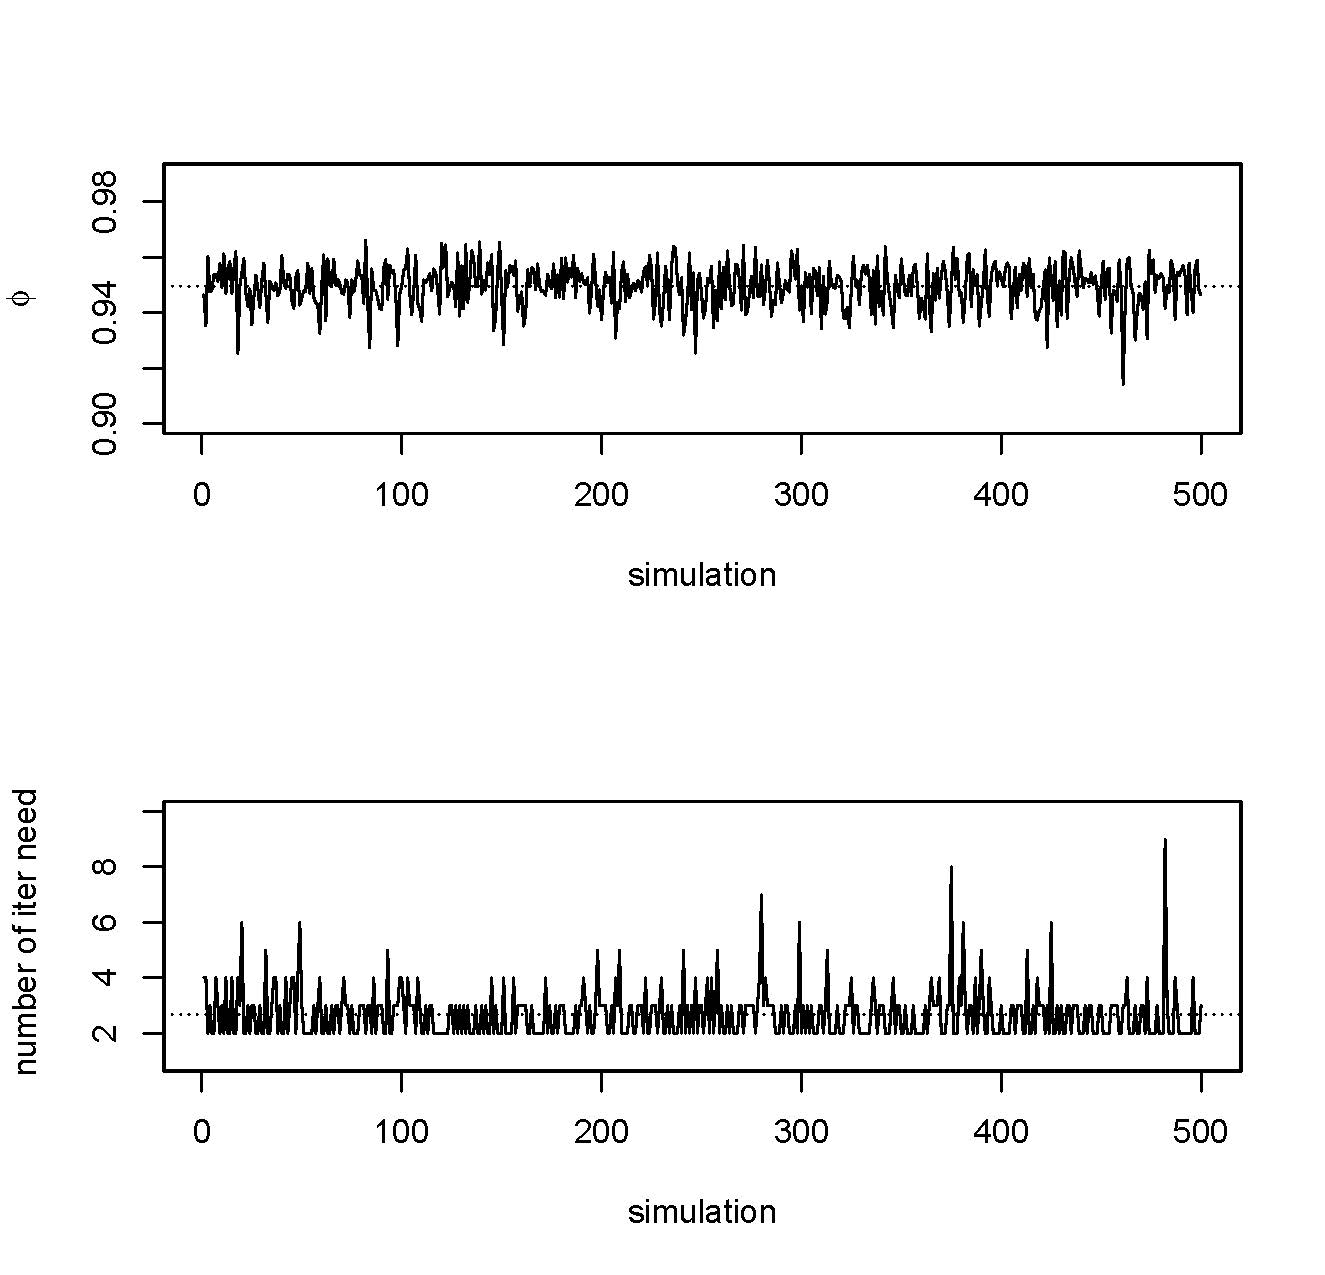
\includegraphics[width=1.0\linewidth]{scoremethod_phi.jpg}
    \caption
    {Estimated results for $\phi$ by Newton optimisation. Top: estimated value of parameter. Bottom:  number of iterations to converge. The dotted lines are the mean value of 500 simulations.}
    \label{fig:scoremethod_phi}
\end{figure}

\begin{figure}[H]
    \centering
    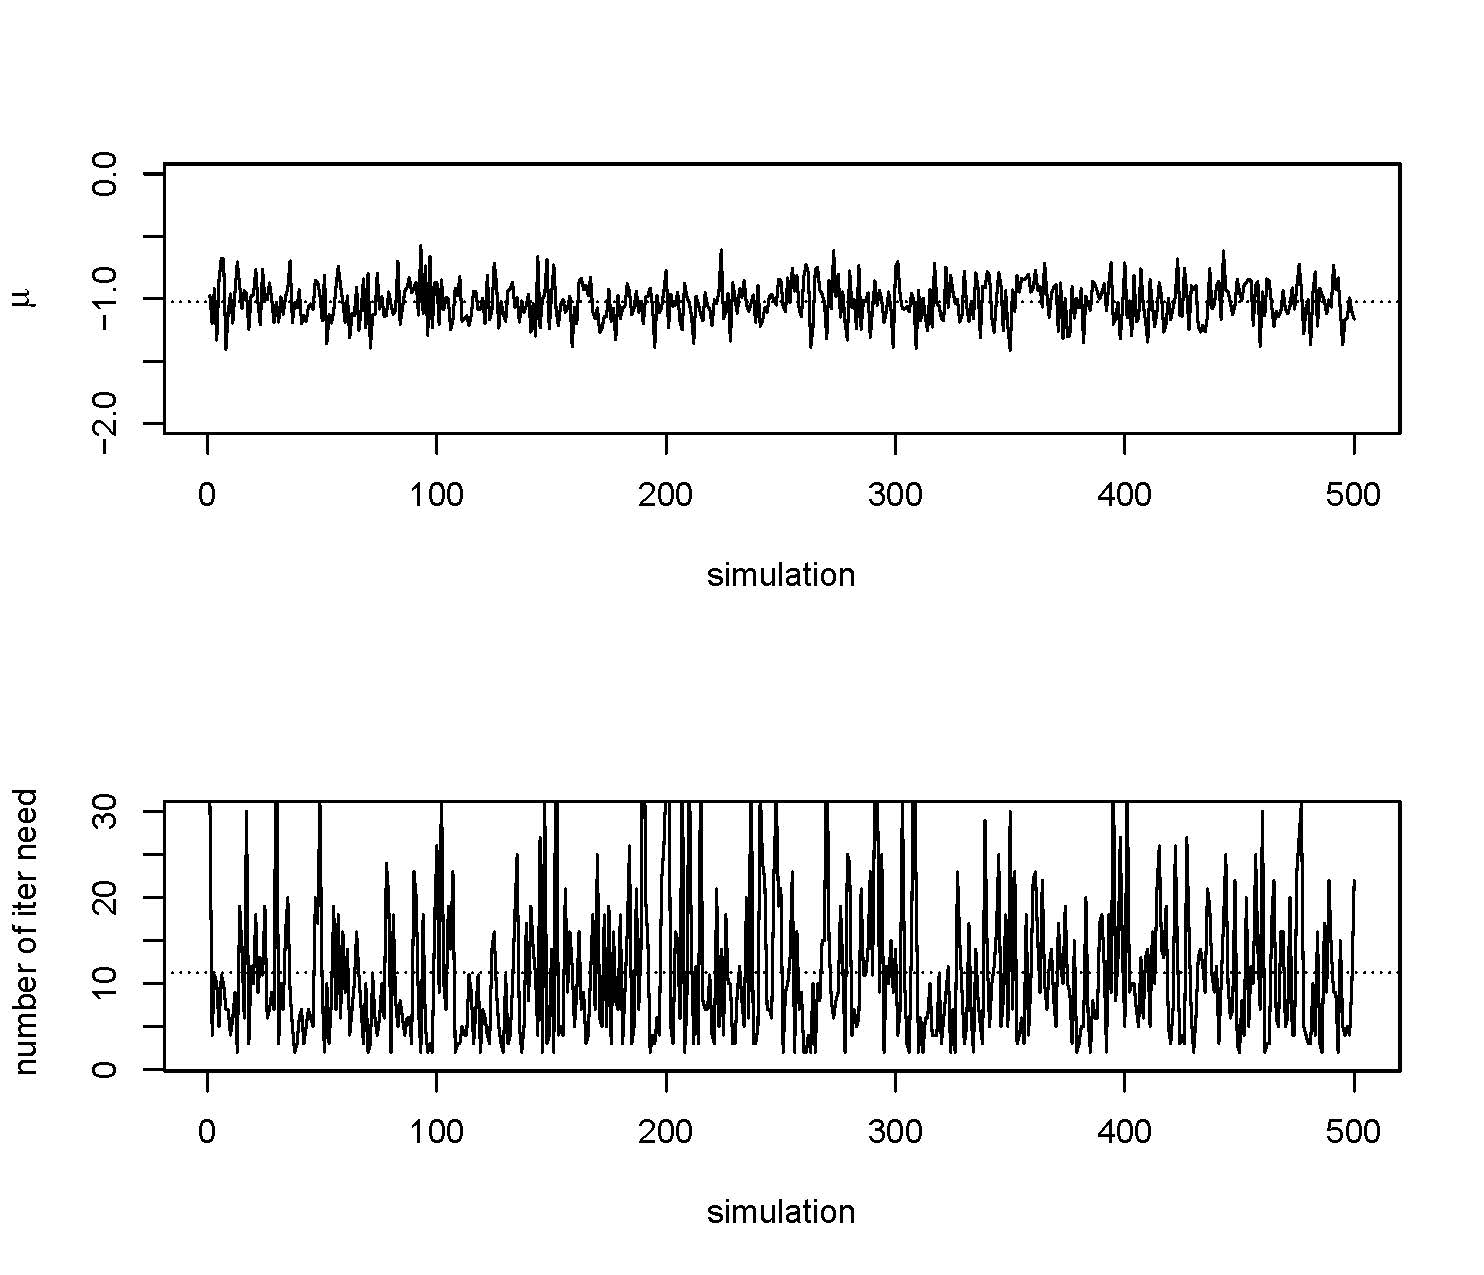
\includegraphics[width=1.0\linewidth]{scoremethod_mu.jpg}
    \caption
    {Estimated results for $\mu$ by Newton optimisation. Top: estimated value of parameter. Bottom:  number of iterations to converge. The dotted lines are the mean value of 500 simulations.}
    \label{fig:scoremethod_mu}
\end{figure}


\chapter{Conclusion}\label{ccl}
We have described the Particle Filter algorithm  to get the Monte Carlo approximation of the latent state in State Space models. What's more, in parameter inference problems, we apply this method to approximate the likelihood, score function and  Hessian matrix and thus get the  maximum likelihood estimation of the unknown parameter  vector by Newton optimisation.\\

\noindent However, there are some topics we do not finish as planned and can be investigated in the future.
We have tried the LGSS model and SV model in this thesis and the next step we planned is to work on the COGARCH model, which doesn't have a tractable log-likelihood. \\

\noindent The particle algorithm we implement in this thesis to 
compute the score function and Hessian matrix is from
the paper \cite{poyiadjis2011particle}. This paper also introduces another particle algorithm which has higher computational complexity but some other advantages. 
What we can do in future is to apply the second algorithm
in ML parameter inference problems and compare the two methods.








%%%%%%%%%%%%%%%%%%%%%%%%%%%%%%%%%%%%%%%%%%%%%%%%%%%%%%%%%%%%%%%%%%%%%%%%%%

\clearpage
\addcontentsline{toc}{chapter}{References}
\bibliographystyle{unswthesis}

\begin{thebibliography}{999}

\bibitem
{cappe2006inference} Capp{\'e}, Olivier and Moulines, Eric and Ryd{\'e}n, Tobias, Inference in hidden Markov models, 
\textit{Springer Science \& Business Media}, 2006.

\bibitem
{arnaud2001sequential} Arnaud, Doucet and de Freitas, Nando and Gordon, Neil, Sequential Monte Carlo methods in practice,
\textit {Information Science and Statistics (Springer New York, 2001)} 
\textbf(2001).

\bibitem
{elliott2008hidden}  Elliott, Robert J and Aggoun, Lakhdar and Moore, John B, Hidden Markov models: estimation and control,
\textit{Springer Science \& Business Media}
\textbf {29},(2008).
  
\bibitem{west2006bayesian} West, Mike and Harrison, Jeff, Bayesian forecasting and dynamic models
\textit{Springer Science \& Business Media}
\textbf(2006).

\bibitem{durbin2012time} Durbin, James and Koopman, Siem Jan,Time series analysis by state space methods,
\textit{Oxford university press}
\textbf(2012).

\bibitem{langrock2011some} Langrock, Roland, Some applications of nonlinear and non-Gaussian state--space modelling by means of hidden Markov models,
\textit{Journal of Applied Statistics}
\textbf{38},{12},(2011),2955--2970.

\bibitem{berger2013statistical} Berger, James O, Statistical decision theory and Bayesian analysis,
\textit{Springer Science \& Business Media}
\textbf(2013).


\bibitem{robert2007bayesian} Robert, Christian, The Bayesian choice: from decision-theoretic foundations to computational implementation,
\textit {Springer Science \& Business Media}
\textbf(2007).

\bibitem{anderson2012optimal} Anderson, Brian DO and Moore, John B, Optimal filtering,
\textit{Courier Corporation} 
\textbf(2012).

\bibitem{stigler1981gauss} Stigler, Stephen M, Gauss and the invention of least squares,
\textit{The Annals of Statistics}
\textbf(1981),465--474.

\bibitem{agrawal2018rewriting} Agrawal, Akshay and Verschueren, Robin and Diamond, Steven and Boyd, Stephen, A rewriting system for convex optimization problems,
\textit{Journal of Control and Decision}
\textbf {5}(1),(2018),42--60.



\bibitem {wiener1949extrapolation}
Wiener, Norbert, Extrapolation, interpolation, and smoothing of stationary time series, vol. 2,
\textit {MIT press Cambridge, MA}
\textbf (1949).
 
\bibitem{kolmogoroff1941interpolation} Kolmogoroff, A, Interpolation und extrapolation von stationaren zufalligen folgen,
\textit{Izvestiya Rossiiskoi Akademii Nauk. Seriya Matematicheskaya} 
\textbf{5}(1),(1941),3--14.




 
\bibitem {kalman1960new} Kalman, Rudolph Emil,
A new approach to linear filtering and prediction problems,
1960.

\bibitem {bucy1971digital} Bucy, Richard S and Senne, Kenneth D,
Digital synthesis of non-linear filters,
\textit{Automatica}
\textbf{7}(3),(1971),287--298.

\bibitem{sunahara1970approximate} Sunahara, Yoshifumi,
An approximate method of state estimation for nonlinear dynamical systems,
(1970).



\bibitem{julier1997new} Julier, Simon J and Uhlmann, Jeffrey K,
New extension of the Kalman filter to nonlinear systems,
\textit{Signal processing, sensor fusion, and target recognition VI}
\textbf{3068},(1997),182--193.


\bibitem{gordon1993novel} Gordon, Neil J and Salmond, David J and Smith, Adrian FM,
Novel approach to nonlinear/non-Gaussian Bayesian state estimation,
\textit{IEE proceedings F (radar and signal processing)}
\textbf{140}(2),(1993),107--113.



\bibitem{ho1964bayesian} Ho, YC and Lee, RCKA,
A Bayesian approach to problems in stochastic estimation and control,
\textit{IEEE transactions on automatic control}
\textbf{9}(4),(1964),333--339.

\bibitem{hammersley1954poor}
Hammersley, John M and Morton, K William,
Poor man's monte carlo,
\textit{Journal of the Royal Statistical Society: Series B (Methodological)}
\textbf{16}(1),(1954), 23--38.



\bibitem{marshall1954use}Marshall, Andrew W,
The use of multi-stage sampling schemes in Monte Carlo computations,
\textit{RAND CORP SANTA MONICA CALIF}
\textbf(1954).

\bibitem{kong1994sequential} Kong, Augustine and Liu, Jun S and Wong, Wing Hung,
Sequential imputations and Bayesian missing data problems,
\textit{Journal of the American statistical association}
\textbf{89}(425),(1994),278--288.

\bibitem{kong1992note} Kong, Augustine,
A note on importance sampling using standardized weights,
\textit{University of Chicago, Dept. of Statistics, Tech. Rep}
\textbf{348},(1992).


\bibitem{liu1998sequential}Liu, Jun S and Chen, Rong,
Sequential Monte Carlo methods for dynamic systems,
\textit{Journal of the American statistical association}
\textbf{93}(443),(1998),1032--1044.


\bibitem{bolic2005resampling} Bolic, Miodrag and Djuric, Petar M and Hong, Sangjin,
Resampling algorithms and architectures for distributed particle filters,
\textit{IEEE Transactions on Signal Processing}
\textbf{53}(7),(2005),2442--2450.

\bibitem{fox2003adapting}Fox, Dieter,
Adapting the sample size in particle filters through KLD-sampling,
\textit{The international Journal of robotics research}
\textbf{22}(12),(2003),985--1003.


\bibitem{sankaranarayanan2008algorithmic}
Sankaranarayanan, Aswin C and Srivastava, Ankur and Chellappa, Rama,
Algorithmic and architectural optimizations for computationally efficient particle filtering,
\textit{IEEE Transactions on Image Processing}
\textbf{17}(5),(2008),737--748.
  
\bibitem{li2012deterministic} Li, Tiancheng and Sattar, Tariq Pervez and Sun, Shudong,
Deterministic resampling: unbiased sampling to avoid sample impoverishment in particle filters,
\textit{Signal Processing}
\textbf{92}(7),(2012),1637--1645.

\bibitem{balasingam2011efficient}
Balasingam, Balakumar and Boli{\'c}, Miodrag and Djuri{\'c}, Petar M and Miguez, Joaquin,
Efficient distributed resampling for particle filters,
\textit{2011 IEEE International Conference on Acoustics, Speech and Signal Processing (ICASSP)}
(2011),3772--3775.


\bibitem{poyiadjis2011particle}
Poyiadjis, George and Doucet, Arnaud and Singh, Sumeetpal S,
Particle approximations of the score and observed information matrix in state space models with application to parameter estimation,
\textit{Biometrika}
\textbf{98}(1),(2011),65--80.

\bibitem{yildirim2015parameter}
Y{\i}ld{\i}r{\i}m, Sinan and Singh, Sumeetpal S and Dean, Thomas and Jasra, Ajay,
Parameter estimation in hidden Markov models with intractable likelihoods using sequential Monte Carlo,
\textit{Journal of Computational and Graphical Statistics}
\textbf{24}(3),(2015),846--865.


\bibitem{del2010forward}
Del Moral, Pierre and Doucet, Arnaud and Singh, Sumeetpal,
Forward smoothing using sequential Monte Carlo,
\textit{arXiv preprint arXiv:1012.5390}
(2010).


\bibitem{lindsten2013backward}
Lindsten, Fredrik and Sch{\"o}n, Thomas B,
Backward simulation methods for Monte Carlo statistical inference,
\textit{Foundations and Trends{\textregistered} in Machine Learning}
\textbf{6}(1),(2013),1--143.

\bibitem{schon2011system}
Sch{\"o}n, Thomas B and Wills, Adrian and Ninness, Brett,
System identification of nonlinear state-space models,
\textit{Automatica}
\textbf{47}(1),(2011),39--49.

\bibitem{chopin2013smc2}
Chopin, Nicolas and Jacob, Pierre E and Papaspiliopoulos, Omiros,
SMC2: an efficient algorithm for sequential analysis of state space models,
\textit{Journal of the Royal Statistical Society: Series B (Statistical Methodology)}
\textbf{75}(3),(2013),397--426.

\bibitem{rue2009approximate}
Rue, H{\aa}vard and Martino, Sara and Chopin, Nicolas,
Approximate Bayesian inference for latent Gaussian models by using integrated nested Laplace approximations,
\textit{Journal of the royal statistical society: Series b (statistical methodology)}
\textbf {71}(2),(2009),319--392.

 
\bibitem {bishop2006pattern}
Bishop, Christopher M,
Pattern recognition and machine learning,
\textit{Springer}
2006.  

\bibitem{minka2013expectation}
Minka, Thomas P,
Expectation propagation for approximate Bayesian inference,
\textit{arXiv preprint arXiv:1301.2294}
(2013).

\bibitem{dahlin2019getting}
Dahlin, Johan and Sch{\"o}n, Thomas B,
Getting started with particle Metropolis-Hastings for inference in nonlinear dynamical models,
\textit{Journal of Statistical Software}
\textbf{88}(CN2),(2019),1--41.


\bibitem{hull1987pricing} Hull, John and White, Alan,
The pricing of options on assets with stochastic volatilities,
\textit{The journal of finance}
\textbf{42}(2),(1987),281--300.

\bibitem{hull2009options}
Hull, John C,
Options, Futures, and other Derivatives (ed.),
\textit{Upper Saddle River, NJ: Prentice Hall},
2009





\end{thebibliography}




\end{document}





